\documentclass{article} %Classe del documento
\usepackage{float}  %Permette di posizionare le immagini dove si vuole
\usepackage{amsmath} %Permette di usare comandi matematici avanzati
\usepackage{booktabs} %Permette di creare tabelle con linee orizzontali
\usepackage[svgnames]{xcolor} %Permette di usare i colori
\usepackage{listings} %Permette di inserire codice R nel documento
\usepackage{upquote} %Permette di usare i singoli apici
\usepackage{graphicx} %Permette di inserire immagini
\usepackage{verbatim} %Permette di inserire commenti multiriga
\usepackage[a4paper, left=1.60in, right=1.60in, top=1.7in, bottom=1.7in]{geometry}
%\usepackage[a4paper, margin=1.6in]{geometry}
\usepackage{changepage} %Permette di regolare i margini
\usepackage[utf8]{inputenc} %Permette l'uso dei caratteri accentati
\usepackage[italian]{babel} %Permette l'uso della la lingua italiana
\usepackage{setspace}   %Permette di regolare la spaziatura
\usepackage{graphicx} %Permette di inserire immagini
\usepackage{tabularx}   %Permette di creare tabelle con larghezza fissa
\usepackage{caption}   %Permette di personalizzare le didascalie
% \usepackage{fancyhdr} %Permette di personalizzare l'intestazione e il piè di pagina
\usepackage{titling} %Permette di personalizzare il titolo

\begin{document}

%Aggiunge spaziatura di 1.5
\setstretch{1.25}

% \maketitle

\begin{titlepage}
    \centering
    % \vspace*{2cm} % Spazio dall'alto
    \vspace{1.5cm}
    {\huge \textbf{Università degli Studi di Padova} \par}
    {\LARGE Dipartimento di Scienze Statistiche \par}
    \vspace{0.5cm}

    {\Large Corso di Laurea Triennale in \par}
    {\Large Statistica per le Tecnologie e le Scienze \par}
    \vspace{1.5cm}

    % Logo
    
\includegraphics[width=0.3\textwidth]{immagini/unipd.png} % Inserisci qui il percorso del logo
    \vspace{1.3cm}

    % Titolo
    % {\Large \textbf{CASO DI STUDIO:}}
    {\Huge Analisi del dataset \texttt{Mussels} \par}

    \vspace{3cm}
    \begin{flushright}
        {\Large \textbf{Relazione di:} \par}
        {\Large Stefano Terrone \par}
        {\Large Leonardo Perin \par}
        \vspace{2cm}
    \end{flushright}
        {\Large \textbf{Anno accademico:} \\2024/2025 \par}
    % \vspace{3cm}

\end{titlepage}

\newpage
\begin{flushleft}
    %\vskip 50pt
\textbf{\Large 0.1 \: Introduzione}    
\end{flushleft}
% \vskip 10pt

Il dataset \texttt{mussels}\textit{[1]} contiene le misurazioni di varie specie di molluschi bivalvi  in 44 fiumi facenti parte della East Coast degli Stati Uniti d'America.\\ 
Il termine “mussels” è un termine generico che indica varie famiglie di molluschi bivalvi, sia di acqua dolce che di acqua salata, che hanno in comune un guscio allungato e asimmetrico\textit{[2]}. In particolare, nello studio sono state analizzate 79 specie di molluschi, appartenenti alla sottoclasse dei \textit{Palaeoheterodonta} e alla famiglia delle \textit{Unionidae}, detti anche cozze di acqua dolce. 
I fiumi osservati fanno parte della costa orientale e sud-orientale degli USA e comprendono i fiumi tra la baia di St. Lawrence e lo stato dell'Alabama. Dunque, sono presenti sia fiumi che sfociano nell'Atlantico orientale, sia i fiumi che sfociano nel Golfo del Messico \textit{(Figura 1)}. 

\begin{figure}[H]
    \centering
    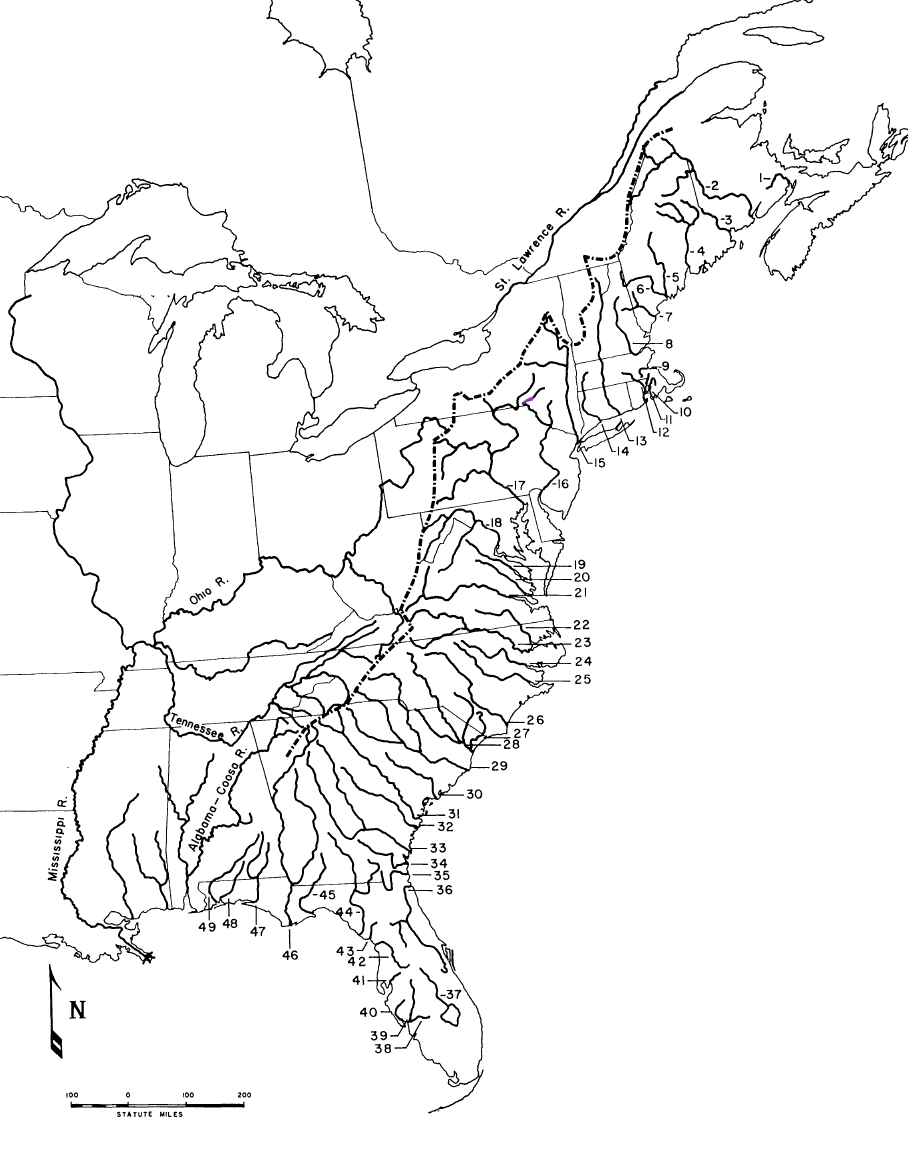
\includegraphics[width=0.58\textwidth]{immagini/usa.png}
    % \captionsetup{justification=centering}
    \caption{Mappa degli Stati Uniti orientali con i fiumi analizzati da \textit{Distribution of Freshwater Mussels: Coastal Rivers as Biogeographic Islands}, di Sepkoski J.J e Michael A., 1974, Systematic Biology. La linea in grassetto tratteggiata è lo spartiacque continentale orientale; confine dell'area in analisi. I numeri sulla mappa sono i fiumi: 4. Penobscot, 5. Kennebec, 6. Androscoggin, 7. Saco, 8. Merrimac, 11. Blackstone, 12. Thames, 13. Connecticut, 14. Housatonic, 15. Hudson, 16. Delaware, 17. Susquehanna, 18. Potomac, 19. Rappahannock, 20. York, 21. James, 22. Chowan, 23. Roanoke, 24. Pamlico, 25. Neuse, 26. Cape Fear, 27. Waccamaw, 28. Pee Dee, 29. Coop-er-Santee, 30. Edisto, 31. Savannah, 32. Ogeechee, 33. Altamaha, 34. Satilla, 35. St. Marys, 36. St. Johns,Fla., 37. Kissimmee, 38. Alafia, 39. Peace, 40. Myakka, 41. Hillsborough, 42. Withlacoochee, 43. Waccasassa, 44. Suwannee, 45. Ochlockonee, 46. Apalachicola, 47. Choctawhatchee, 48. Yellow, 49. Escambia.}
\end{figure}


Lo scopo di questo studio è valutare quali fattori influiscano sul numero di specie di cozze in un fiume. Per fare ciò sono state osservate altre 9 variabili come il numero totale di specie di cozze presenti in un fiume, l'area totale del fiume, la distanza da fiumi principali e anche fattori di qualità delle acque. 
La variabile \texttt{Species} è il numero di specie di cozze presenti nel fiume osservato. 
La variabile \texttt{Area} è la misurazione in \textit{miglia quadrate} dell'area di drenaggio di un fiume. L'area è stata misurata usando un planimetro polare su una mappa sulle risorse idriche \textit{(Figura 1)} fornita dal dipartimento sulla geologia degli USA \textit{(USGS)}.  
La variabile \texttt{ln(Area)} è il logaritmo naturale dell'area del fiume.
Per valutare la dispersione delle specie di cozze nell'area geografica di riferimento, si è deciso di designare alcuni fiumi come fiumi di origine delle varie specie di cozze. 
I fiumi scelti sono: il sistema fluviale dell'Alabama-Coose \textit{(AC)}, il fiume Apalachicola \textit{(AP)}, il fiume Savannah \textit{(SV)}, e il fiume St. Lawrence \textit{(SL)}. I primi due fiumi (AP e AC) sfociano nel Golfo del Messico, mentre gli altri due (SV e SL) sfociano nell'Atlantico orientale. Altri criteri che hanno deciso la scelta dei fiumi sono: importanza geografica, numero di specie di cozze presenti e la loro dispersione nei fiumi limitrofi. Data la irregolarità del corso di un fiume, al fine di misurare la distanza dei fiumi osservati dai 4 fiumi principali, non è stata usata una misura lineare della distanza, ma si è deciso di misurare la distanza in termini di prossimità. Viene così sfruttata la caratteristica dei fiumi di scorrere in modo lineare lungo la costa. Ogni fiume viene quindi visto come il passo di un saltello, e la distanza viene stimata semplicemente contando quanti fiumi separano il fiume osservato da quelli principali. Le variabili che misurano la distanza sono 4: 
\texttt{Stepping stones to AC}, ovvero i “saltelli” necessari a raggiungere il sistema fluviale Alabama-Coosa; 
\texttt{Stepping stones to AP}, “saltelli” dal fiume Apalachicola; 
\texttt{Stepping stones to SL}, “saltelli” dalla foce del fiume St. Lawrence e, infine, 
\texttt{Stepping stones to SV}, “saltelli” dalla foce del fiume Savannah.
Per valutare la qualità delle acque sono state misurate tre variabili: 
\texttt{Nitrate}, che rappresenta la concentrazione in \textit{parti per milione} di nitrato \texttt{NO\textsubscript{3}}\textit{[3]} nelle acque del fiume. Questo ione è fondamentale per la produzione di alghe e batteri che rappresentano la principale fonte di cibo per le cozze\textit{[4]}; 
\texttt{Solid Residue}, che rappresenta il residuo fisso nelle acque, ovvero la quantità in \textit{parti per milione} di sali minerali e oligoelementi presenti in soluzione o sospensione nell'acqua del fiume. Questa variabile è stata misurata facendo prima evaporare l'acqua a 180\textsuperscript{o} C per una ora e, successivamente, pesando ciò che rimane. Risulta utile perchè permette di valutare la concentrazione di alcuni sali come il sodio, il potassio, il calcio e il magnesio e la salinità delle acque; 
\texttt{Hydronium}, è la concentrazione in \textit{grammi-ioni per $10^7$} di idronio (\textit{H\textsubscript{3}O\textsuperscript{+}}) nell'acqua\textit{[6]}. Questa quantità è ottenuta tramite l'operazione inversa del calcolo del pH e rappresenta l'antilogaritmo in base 10 del suo negativo. Questa misurazione torna utile in quanto il pH, e in particolare la presenza dello ione idrogeno (\textit{H\textsuperscript{+}}), è un importante fattore nella calcificazione del guscio delle cozze\textit{[5]}. Non viene misurato direttamente lo ione idrogeno (detto anche idrone) perchè non può esistere in soluzione acquosa allo stato libero. \\
Le analisi sono state eseguite con il software R nella versione 4.2.3 \\\textit{(https://www.r-project.org/)}.\\ Il livello di significatività è fissato al 5\%.

% \vskip 55pt 

%\newpage
\begin{flushleft}
    \vskip 30pt
    \textbf{\Huge 1. \: Analisi esplorative}
    \vskip 30pt
    %Prima parte: analisi univariate
    %Titolo
    \textbf{\Large 1.1 \: Analisi Univariate}
\end{flushleft}
\vskip 10pt

%Introduzioni analisi esplorative
Il database è composto da 44 osservazioni, una per ciascun fiume, e 9 varabili. 
Le varabili sono riportate in \textit{Tabella 1}.

%Tabella di sintesi
\begin{table}[H]
    \centering
    \renewcommand{\arraystretch}{1.4} % Increases the row height
    \begin{tabularx}{\textwidth}{p{69pt}l p{30pt}c p{45pt}c p{35pt}c p{40pt}c p{30pt}c p{27pt}r}
        \toprule
        & Min. & 1\textsuperscript{o} qt. & Mediana(IQR) & Media(sd) & 3\textsuperscript{o} qt. & Max\\
            \midrule  
            \texttt{Species} & 2.00 & 8.00 & 10.00(5.0) & 11.25(5.99) & 13.00 & 33.00 \\
            \texttt{Area} & 349 & 2115 & 4315(7797.5) & 6590(6016) & 9912 & 27900 \\
            \texttt{Stepping}\\ \texttt{stones to AC} & 1.00 & 7.00 & 15.50(15.25) & 15.34(9.19) & 22.25 & 33.00 \\
            \texttt{Stepping }\\
            \texttt{stones to AP} & 0.00 & 4.00 & 12.00(14.25) & 12.02(8.24) & 18.25 & 28.00 \\
            \texttt{Stepping }\\
            \texttt{stones to SV} & 0.00 & 5.00 & 7.00(13.25) & 8.136(8.94) & 11.00 & 21.00 \\
            \texttt{Stepping }\\
            \texttt{stones to SL} & 4.00 & 16.75 & 22.00(0.775) & 22.16(1.84) & 30.00 & 36.00 \\
            \texttt{Nitrate} & 0.100 & 0.600 & 0.800(0.775) & 1.495(1.84) & 1.375 & 8.700 \\
            \texttt{Solid Residue} & 29.0 & 56.5 & 78.0(64.0) & 112.4(17.3) & 120.5 & 520.0 \\
            \texttt{Hydronium} & 0.200 & 1.00 & 1.600(2.2) & 3.631(6.03) & 3.200 & 32.00 \\
            \texttt{ln(Area)} & 5.855 & 7.657 & 8.370(1.54) & 8.331(1.07) & 9.201 & 10.24 \\
        \bottomrule
    \end{tabularx}
    \caption{Tabella di sintesi delle variabili del dataset}
\end{table}

\begin{figure}[H]
    \centering
    \begin{minipage}{0.49\textwidth}
        \centering
        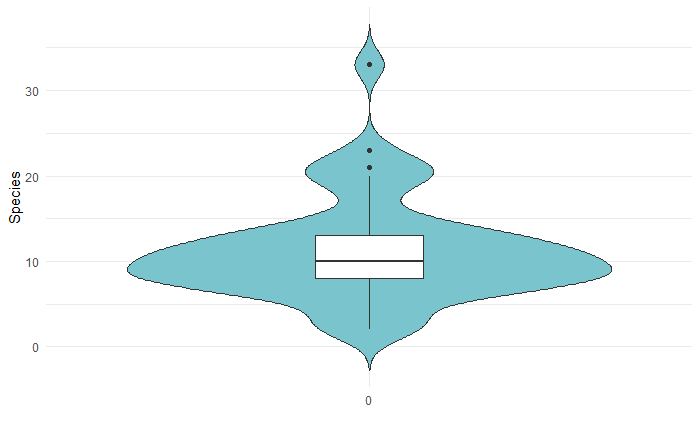
\includegraphics[width=\textwidth]{immagini/vp_species.png}
        \captionsetup{justification=centering}
        \caption{Violinplot della variabile \texttt{Species}}
    \end{minipage}
    \hfill
    \begin{minipage}{0.49\textwidth}
        \centering
        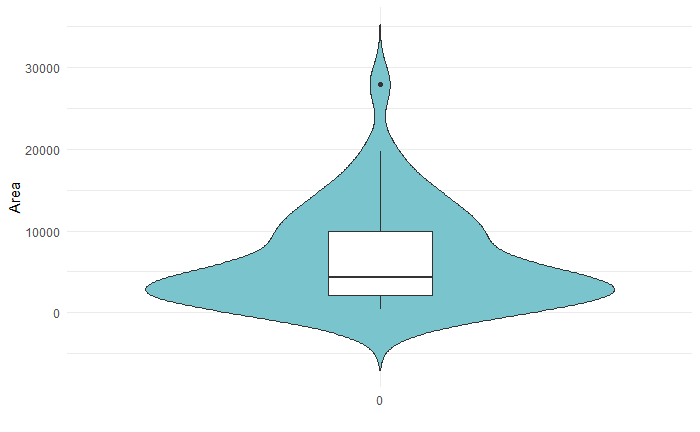
\includegraphics[width=\textwidth]{immagini/vp_area.png}
        \captionsetup{justification=centering}
        \caption{Violinplot della variabile\\ \texttt{Area}}
    \end{minipage}
\end{figure}

La variabile \texttt{Species}, rappresentante il numero di specie di cozze nel fiume, ha una distribuzione asimmetrica a destra 
come evidenziato dal violinplot \textit{(Figura 2)}. Sono presenti 4 outliers: i fiumi Cooper-Santee e Savannah con 21 specie, il fiume Escambia con 23 specie e il fiume Apalachicola con 33 specie. \texttt{Species} ha un valore minimo di 2 specie (nel fiume Waccasassa) e un massimo di 33 specie (nel fiume Apalachicola). La mediana è di 10 specie, la media è di 11.25 specie.

La variabile \texttt{Area} segue una distribuzione asimmetrica a destra \textit{(Figura 3)}, con un valore minimo di 349 \textit{sq mi (square mile)} e un massimo di 27900 \textit{sq mi}, corrispondente al fiume Susquehanna, che rappresenta l'unico outlier. La mediana è di 4315 \textit{sq mi}, la media è di 6590 \textit{sq mi} \textit{(Tabella 1)}.

\begin{figure}[H]
    \centering
    \begin{minipage}{0.49\textwidth}
        \centering
        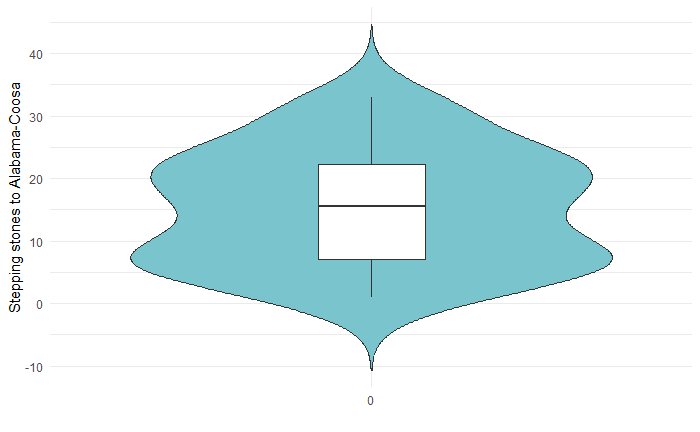
\includegraphics[width=\textwidth]{immagini/vp_ac.png}
        \captionsetup{justification=centering}
        \caption{Violinplot della variabile \texttt{Stepping stones to AC}}
    \end{minipage}
    \hfill
    \begin{minipage}{0.49\textwidth}
        \centering
        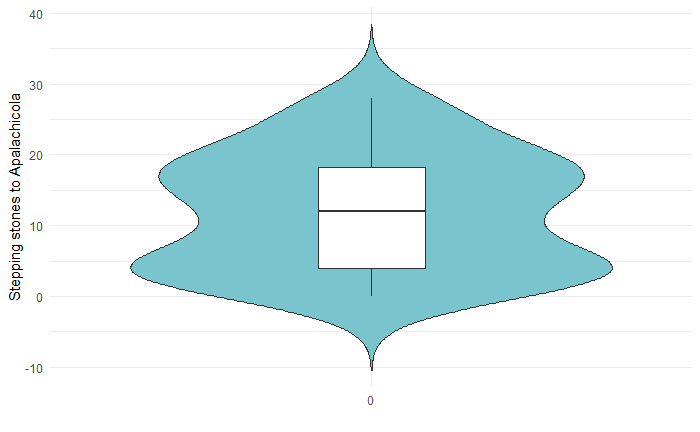
\includegraphics[width=\textwidth]{immagini/vp_ap.png}
        \captionsetup{justification=centering}
        \caption{Violinplot della variabile \texttt{Stepping stones to AP}}
    \end{minipage}
\end{figure}
La distanza dal sistema fluviale di Alabama-Coose (\texttt{Stepping stones to AC}) segue una distribuzione simmetrica \textit{(Figura 4)}, suggerendo che i fiumi sono equamente distribuiti rispetto a questo sistema fluviale. La distanza minima è di 1 e la massima di 33. La distanza media è di 15.34, e quella mediana di 15.50 "saltelli".

Anche la distanza dal fiume Apalachicola (\texttt{Stepping stones to AP}) segue una distribuzione simmetrica \textit{(Figura 5)}, con una distanza minima di 0 (coincidente con il fiume stesso) e una massima di 28. La distanza media è di 12.02, e quella mediana di 12.00 "saltelli" \textit{(Tabella 1)}.

\begin{figure}[H]
    \centering
    \begin{minipage}{0.49\textwidth}
        \centering
        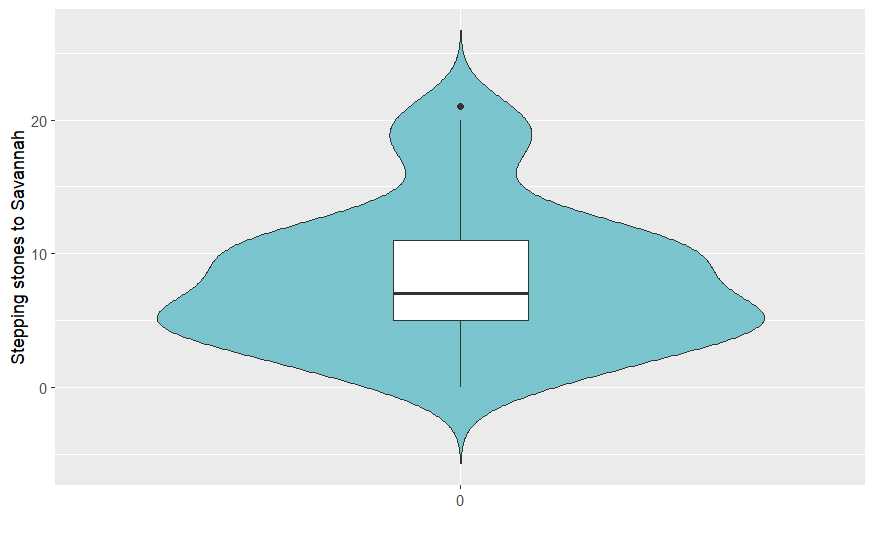
\includegraphics[width=\textwidth]{immagini/vp_sv.png}
        \captionsetup{justification=centering}
        \caption{Violinplot della variabile \texttt{Stepping stones to SV}}
    \end{minipage}
    \hfill
    \begin{minipage}{0.49\textwidth}
        \centering
        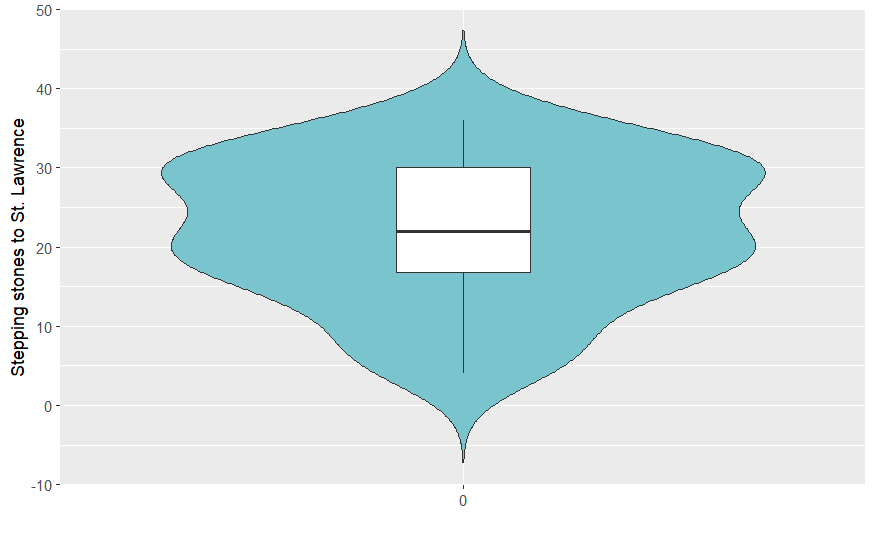
\includegraphics[width=\textwidth]{immagini/vp_sl.png}
        \captionsetup{justification=centering}
        \caption{Violinplot della variabile \texttt{Stepping stones to SL}}
    \end{minipage}
\end{figure}
La distanza dal fiume Savannah (\texttt{Stepping stones to SV}) ha una distribuzione simmetrica anche se presenta una leggera coda lunga a destra \textit{(Figura 6)}, con una distanza minima di 0 (coincidente con il fiume stesso) e una massima di 21, corrispondente al fiume Penobscot, situato a Nord e outlier in figura. La distanza media è di 8.136, e quella mediana di 7.00. Il valore molto basso della mediana e la presenza di una piccola coda lunga a destra suggeriscono che la maggior parte dei fiumi osservati sono molto vicini al fiume Savannah.

La distanza dal fiume St.\ Lawrence (\texttt{Stepping stones to SL}) ha una distribuzione simmetrica \textit{(Figura 7)}, ma presenta anche una leggera coda lunga a sinistra. La distanza minima di 4 e una massima di 36. La distanza media è di 22.16, e quella mediana di 22.00. Il valore elevato della di media e mediana, in aggiunta alla leggera coda a sinistra, suggerisce che la maggior parte dei fiumi sono distanti al fiume St. Lawrence \textit{(Tabella 1)}.


\begin{figure}[H]
    \centering
    \begin{minipage}{0.49\textwidth}
        \centering
        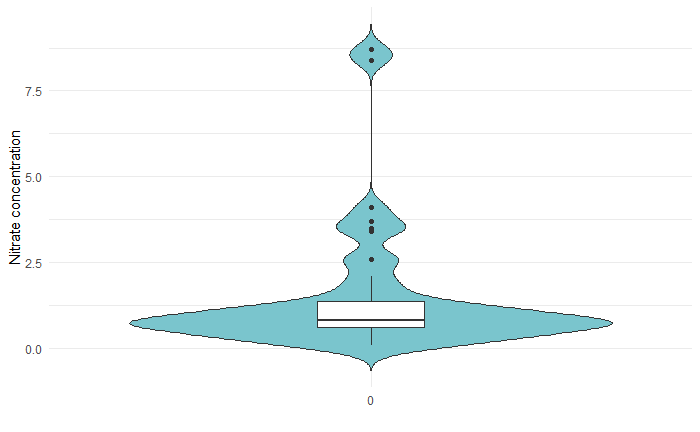
\includegraphics[width=\textwidth]{immagini/vp_nitrate.png}
        \captionsetup{justification=centering}
        \caption{Violinplot della variabile \texttt{Nitrate}}
    \end{minipage}
    \hfill
    \begin{minipage}{0.49\textwidth}
        \centering
        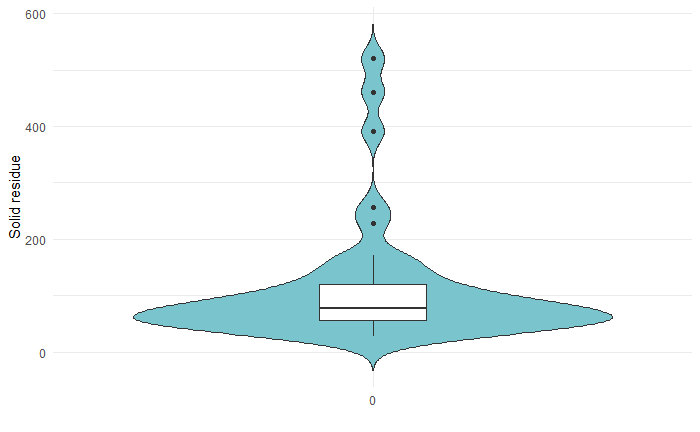
\includegraphics[width=\textwidth]{immagini/vp_sd.png}
        \captionsetup{justification=centering}
        \caption{Violinplot della variabile \texttt{Solid Residue}}
    \end{minipage}
\end{figure}
La variabile \texttt{Nitrate} ha una distribuzione asimmetrica a destra. Sono presenti 6 outliers: i fiumi Susquehanna, Thames, Potomac, Roanoke, Balckstone e Delaware che presentano tutti una elevata concentrazione di nitrato, rispettivamente di 3.4, 3.5, 3.7, 4.1, 8.4 e 8.7 \textit{(Figura 8)}. Il valore minimo è di 0.100 \textit{ppm (parts per million)} e il massimo di 8.700 \textit{ppm}. La mediana è di 0.800 \textit{ppm}, la media è di 1.495 \textit{ppm}.

La variabile \texttt{Solid Residue} ha anche essa una distribuzione asimmetrica a destra. Sono presenti 5 outliers corrispondenti a fiumi con una elevata quantità di residuo fisso nella acque. Essi sono: il Withlacooche (229 \textit{ppm}), il Peace (257 \textit{ppm}), il Waccasassa (461 \textit{ppm}), l'Alafia (520 \textit{ppm}) e il St. Johns, Fla. (391 \textit{ppm}) \textit{(Figura 9)}. La concentrazione minima è di 29.0 \textit{ppm} e la massima di 520.0 \textit{ppm}. La mediana è di 78.0 \textit{ppm}, la media è di 112.4 \textit{ppm} \textit{(Tabella 1)}.


\begin{figure}[H]
    \centering
    \begin{minipage}{0.49\textwidth}
        \centering
        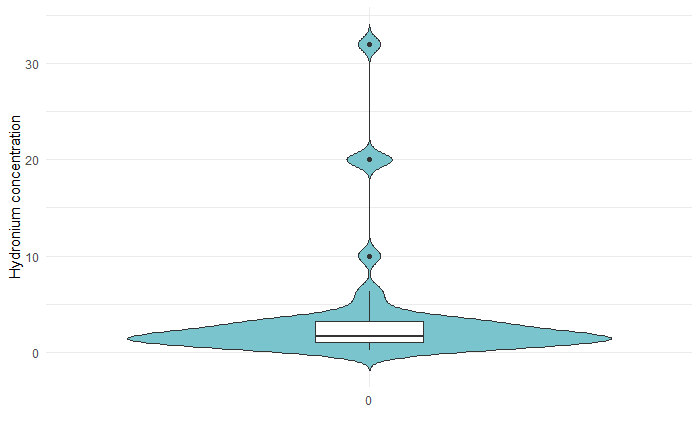
\includegraphics[width=\textwidth]{immagini/vp_hy.png}
        \captionsetup{justification=centering}
        \caption{Violinplot della variabile \texttt{Hydronium}}
    \end{minipage}
    \hfill
    \begin{minipage}{0.49\textwidth}
        \centering
        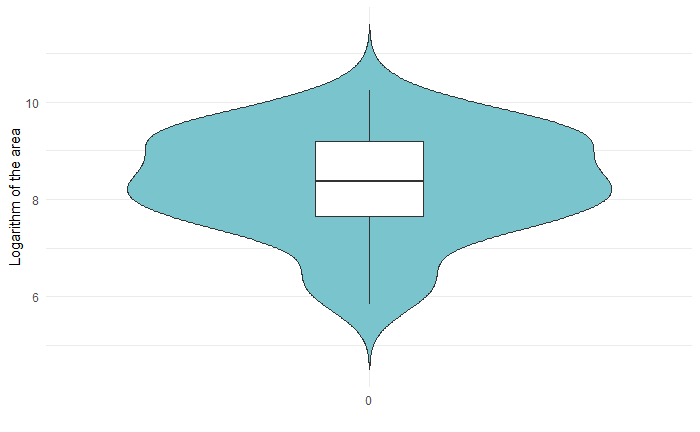
\includegraphics[width=\textwidth]{immagini/vp_ln.png}
        \captionsetup{justification=centering}
        \caption{Violinplot della variabile \texttt{ln(Area)}}
    \end{minipage}
\end{figure}
La variabile \texttt{Hydronium} ha una distribuzione asimmetrica a destra. Sono presenti 4 outliers, tutti corrispondenti a fiumi con una elevata quantità di idronio. I fiumi sono: il Waccamaw, il St. Marys, il Blackstone e il Satilla \textit{(Figura 10)}. Il valore minimo di idronio è di 0.200, il massimo di 32.00. La mediana è di 1.600, la media è di 3.631.

La variabile \texttt{ln(Area)} segue una distribuzione simmetrica \textit{(Figura 11)}, con un valore minimo di 5.855 e un massimo di 10.24. La mediana è di 8.370, la media è di 8.331 \textit{(Tabella 1)}.


%Seconda parte: analisi bivariate
%Titolo
\newpage
\begin{flushleft}
    \textbf{\Large 1.2 \: Analisi Bivariate}
    %\vskip 10pt
\end{flushleft}
\vskip 10pt

%Introduzione analisi bivariate
Si valuta la relazione tra le varie variabili. Delle 36 bivariate totali, 16 bivariate sono risultate significative \textit{(Tabella 2)}.\\

\begin{table}[H]
    \centering
    \renewcommand{\arraystretch}{1.4} % Increases the row height
    % \begin{tabularx}{\textwidth}{p{15pt}l p{20pt}c p{20pt}c p{20pt}c p{20pt}c p{20pt}c p{20pt}r}
    \begin{tabular}{lcccccccc}
        \toprule
        & \texttt{A} & \texttt{H\textsuperscript{+}} & \texttt{SR} & \texttt{NO\textsubscript{3}} & \texttt{SL} & \texttt{SV} & \texttt{AP} & \texttt{AC} \\
        % & & & \texttt{Residue}& & \texttt{stones to SL} & \texttt{stones to SV} & \texttt{stones to AP} & \texttt{stones to AC} &\\
        \midrule  
            \texttt{Sp} & \textcolor{red}{$<$0.001} & 0.411 & 0.638 & 0.514 & 0.334 & 0.862 & 0.299 & 0.347 \\
            \texttt{AC} & 0.246 & \textcolor{red}{0.029} & 0.543 & \textcolor{red}{0.004} & \textcolor{red}{$<$0.001} & \textcolor{red}{$<$0.001} & \textcolor{red}{$<$0.001} \\
            \texttt{AP} & 0.297 & \textcolor{red}{0.026} & 0.479 & \textcolor{red}{0.005} & \textcolor{red}{$<$0.001} & \textcolor{red}{$<$0.001} &  \\
            \texttt{SV} & 0.832 & 0.573 & 0.592 & \textcolor{red}{0.015} & \textcolor{red}{$<$0.001} &  & &  \\
            \texttt{SL} & 0.348 & \textcolor{red}{0.021} & 0.484 & \textcolor{red}{$<$0.001} &  &  &  \\
            \texttt{NO\textsubscript{3}} & 0.462 & 0.403 & \textcolor{red}{$<$0.001} &  &  &  & & \\
            \texttt{SR} & 0.348 & \textcolor{red}{$<$0.001} &  &  &  &  &  \\
            \texttt{H\textsuperscript{+}} & 0.596 &  &  &  &  &  & & \\
        \bottomrule
    \end{tabular}
    % \captionsetup{justification=centering}
    \caption{Tabella che indica la significatività delle correlazioni, in rosso le correlazioni significative.\\
    In particolare Sp: \texttt{Species}, AC: \texttt{Stepping stones to AC}, AP: \texttt{Stepping stones to AP}, SV:\ \texttt{Stepping stones to SV}, SL:\ \texttt{Stepping stones to SL}, NO\textsubscript{3}: \texttt{Nitrate}, SR:\ \texttt{Solid Residue}, H\textsuperscript{+}: \texttt{Hydronium}, A: corrispondente sia a \texttt{Area} che a \texttt{ln(Area)}}
\end{table}

\begin{figure}[H]
    \centering
    \begin{minipage}{0.49\textwidth}
        \centering
        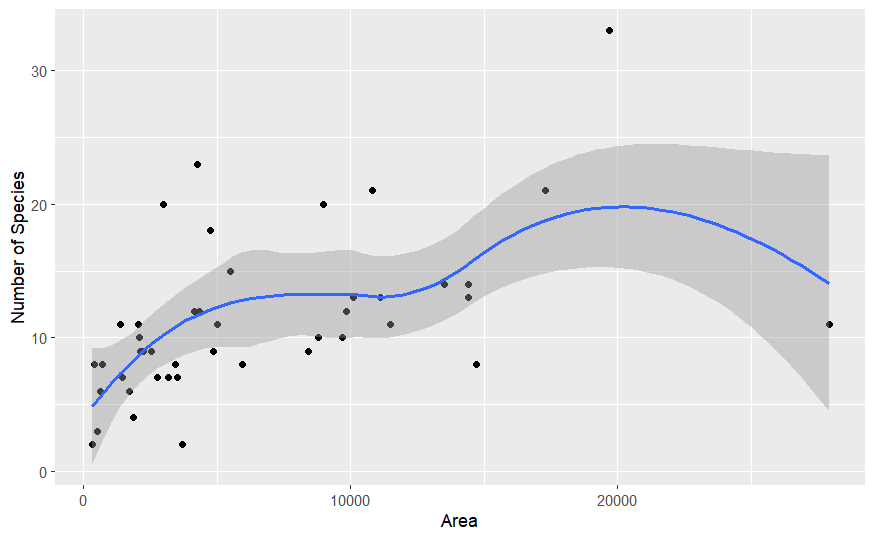
\includegraphics[width=\textwidth]{immagini/sp_a.png}
        \captionsetup{justification=centering}
        \caption{Diagrammma di dispersione tra \texttt{Species} e \texttt{Area}, con curva LOESS \textit{(LOcally Estimated Scatterplot Smoothing)} in blu e intervallo di confidenza al 95\% in grigio}
    \end{minipage}
    \hfill
    \begin{minipage}{0.49\textwidth}
        \centering
        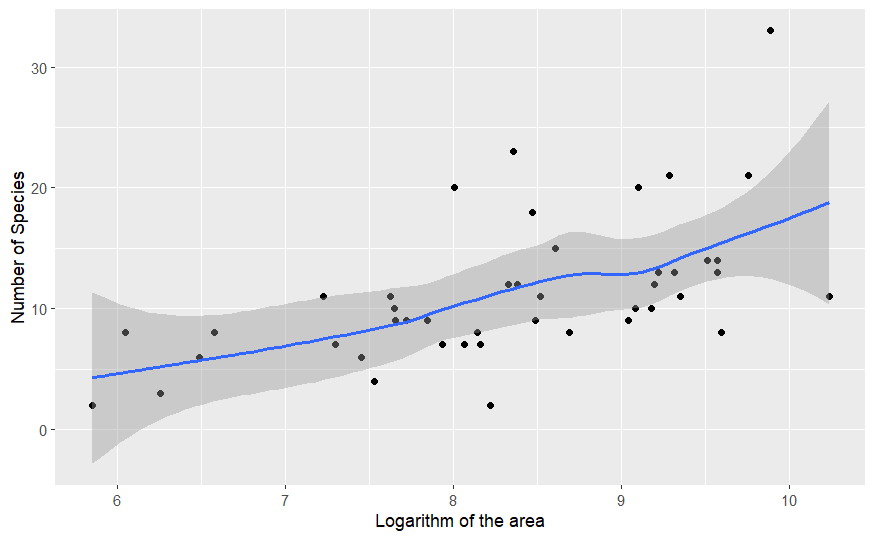
\includegraphics[width=\textwidth]{immagini/sp_ln.png}
        \captionsetup{justification=centering}
        \caption{Diagrammma di dispersione tra \texttt{Species} e \texttt{ln(Area)}, \\con curva LOESS in blu \\e intervallo di confidenza \\al 95\% in grigio}
    \end{minipage}
\end{figure}

Dal diagramma di dispersione tra il numero di specie di cozze e l'area \textit{(Figura 12)} si nota una relazione positiva, ma molto curvilinea tra le due variabili.  
La correlazione di Spearman è 0.64, indicando una relazione positiva tra le due variabili; dunque all'aumentare dell'area del fiume aumenta anche il numero di specie di cozze presenti.
Il test per verificare se la correlazione è significativa (S=5089.2, p-value$<$0.001) porta a rifiutare l'ipotesi che la correlazione non sia significativa che conferma la presenza di una relazione positiva tra le due variabili.

Dal diagramma di dispersione tra il numero di specie di cozze e il logaritmo dell'area \textit{(Figura 13)} si nota una relazione positiva tra le due variabili. La relazione però, appare più lineare rispetto a quella tra l'area e il numero di specie \textit{(Figura 12)}.  
La correlazione di Spearman è 0.64, uguale a quella osservata in precedenza. Le conclusioni sono le stesse: all'aumentare del logaritmo dell'area del fiume aumenta anche il numero di specie di cozze presenti.
Anche il test per verificare se la correlazione è significativa (S=5089.2, p-value$<$0.001) risulta uguale al test fatto precedentemente. Dunque, si rifiuta l'ipotesi che la correlazione non sia significativa.

\begin{figure}[H]
    \centering
    \begin{minipage}{0.49\textwidth}
        \centering
        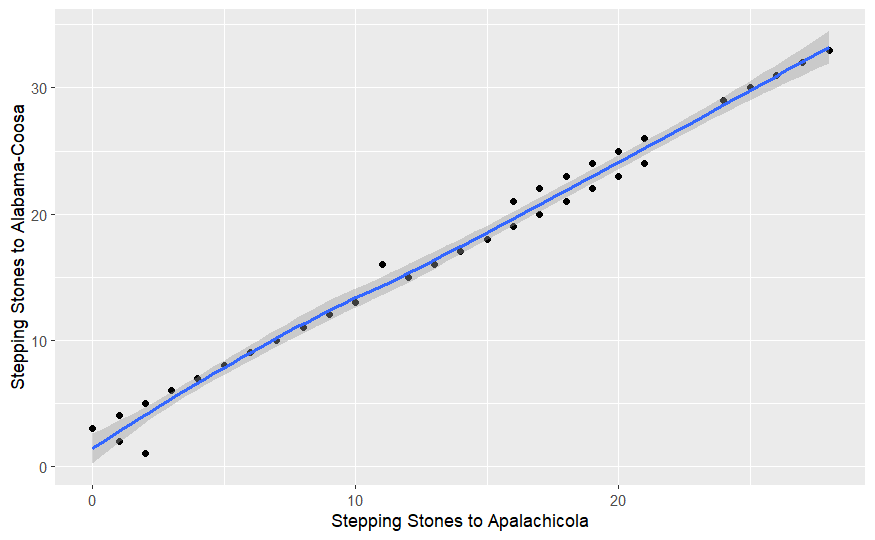
\includegraphics[width=\textwidth]{immagini/ac_ap.png}
        \captionsetup{justification=centering}
        \caption{Diagramma di dispersione tra \texttt{Stepping stones to AC} e \texttt{Stepping stones to AP}, con curva LOESS in blu e intervallo di confidenza al 95\% in grigio}
    \end{minipage}
    \hfill
    \begin{minipage}{0.49\textwidth}
        \centering
        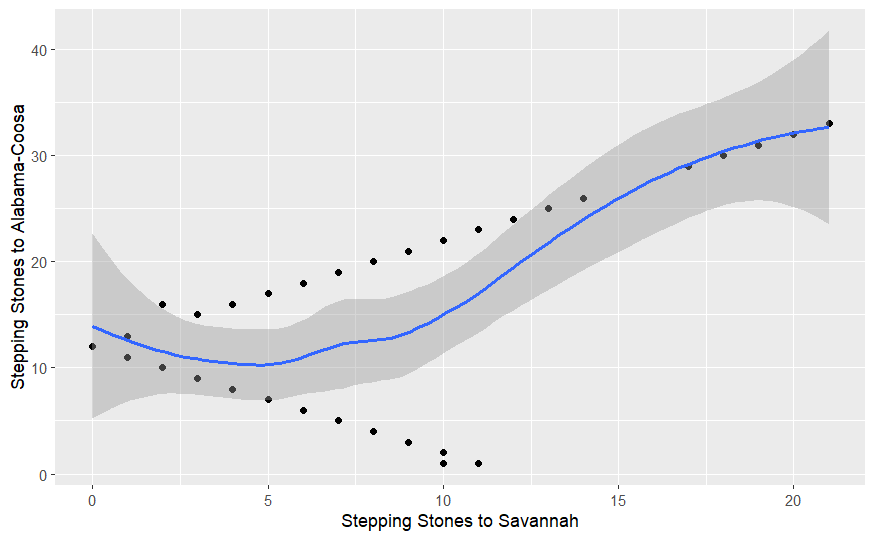
\includegraphics[width=\textwidth]{immagini/ac_sv.png}
        \captionsetup{justification=centering}
        \caption{Diagrammma di dispersione tra \texttt{Stepping stones to AC} e \texttt{Stepping stones to SV}, con curva LOESS in blu e intervallo di confidenza al 95\% in grigio}
    \end{minipage}    
\end{figure}

Dal diagramma di dispersione tra la distanza dei vari fiumi osservati dal sistema fluviale Alabama-Coose e dal fiume Apalachicola \textit{(Figura 14)} si nota una relazione positiva, quasi lineare, tra le due variabili.  
La correlazione di Spearman è 0.99, indicando una forte relazione positiva tra le due variabili; dunque all'aumentare della distanza di un fiume dal sistema fluviale Alabama-Coose aumenta anche la distanza dal fiume Apalachicola. 
Questa relazione è dovuta al fatto che i due fiumi sono molto vicini tra loro, scorrono in parallelo, e sfociano entrambi nel Golfo del Messico, e quindi la distanza da uno implica la distanza dall'altro.
Il test per verificare se la correlazione è significativa (S=89.42, p-value$<$0.001) porta a rifiutare l'ipotesi che la correlazione non sia significativa.

Dal diagramma di dispersione tra la distanza dei vari fiumi osservati dal sistema fluviale Alabama-Coose e dal fiume Savannah \textit{(Figura 15)} si nota una relazione tendenzialmente positiva, ma molto curvilinea tra le due variabili. 
In particolare si nota come nella prima del grafico i punti divergono tra di loro. Questo è dovuto al fatto che il fiume Savannah e il sistema fluviale Alabama-Coose scorrono perpendicolarmente tra di loro, quasi a formare un angolo retto. Quindi una porzione di fiumi (quelli situati a Sud), mentre si allontananano dal fiume Savannah si avvicinano al sistema fluviale Alabama-Coose. Al contrario, i fiumi situati a Nord si allontananano parallamente ad entrambi i fiumi che spiega la crescita positiva nella seconda parte del grafico.
La correlazione di Spearman è 0.54, indicando una modesta relazione positiva tra le due variabili. La correlazione è positiva; dunque all'aumentare della distanza di un fiume dal sistema fluviale Alabama-Coose aumenta anche la distanza dal fiume Savannah. 
Il test per verificare se la correlazione è significativa (S=6483.6, p-value$<$0.001) porta a rifiutare l'ipotesi che la correlazione non sia significativa.

\begin{figure}[H]
    \centering
    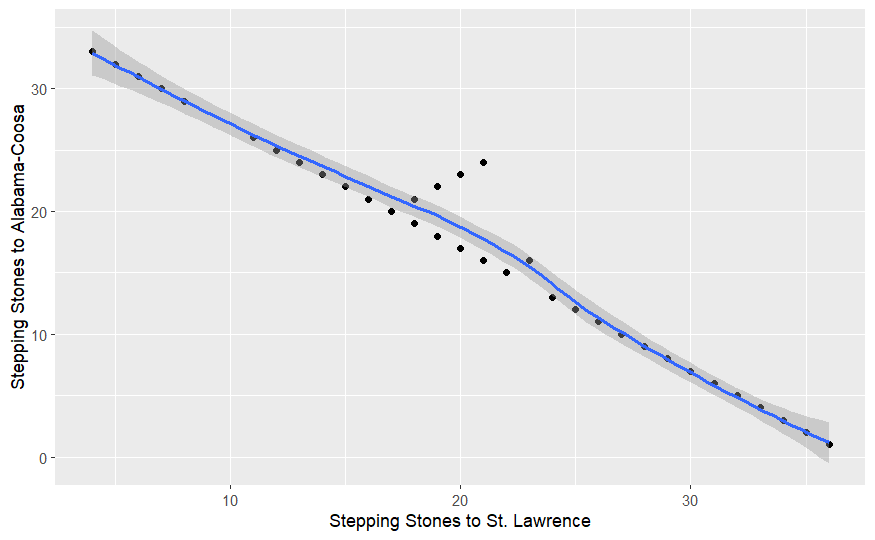
\includegraphics[width=0.5\textwidth]{immagini/ac_sl.png}
    \captionsetup{justification=centering}
    \caption{Diagramma di dispersione tra \\\texttt{Stepping stones to AC} e \texttt{Stepping}\\\texttt{ stones to SL}, con curva LOESS in blu \\e intervallo di confidenza al 95\% in grigio}
\end{figure}

Dal diagramma di dispersione tra la distanza dei vari fiumi osservati dal sistema fluviale Alabama-Coose e dal fiume Saint Lawrence \textit{(Figura 16)} si nota una relazione negativa, abbastanza lineare, tra le due variabili.  
La correlazione di Spearman è \\-0.97, indicando una forte relazione negativa tra le due variabili; dunque all'aumentare della distanza di un fiume dal sistema fluviale Alabama-Coose diminuisce la distanza dal fiume St. Lawrence. 
Questo è dovuto dalla posizione dei due fiumi. Essi, infatti, si trovano alle due estremità della regione osservata, con il fiume St. Lawrence situato a Nord-Est e il sistema fluviale Alabama-Coose situato invece a Sud-Ovest. Quindi allontanandosi dal sistema fluviale Alabama-Coose ci si avvicina al fiume St. Lawrence, e viceversa.
Il test per verificare se la correlazione è significativa (S=28075, p-value$<$0.001) porta a rifiutare l'ipotesi che la correlazione non sia significativa.

\begin{figure}[H]
    \centering
    \begin{minipage}{0.49\textwidth}
        \centering
        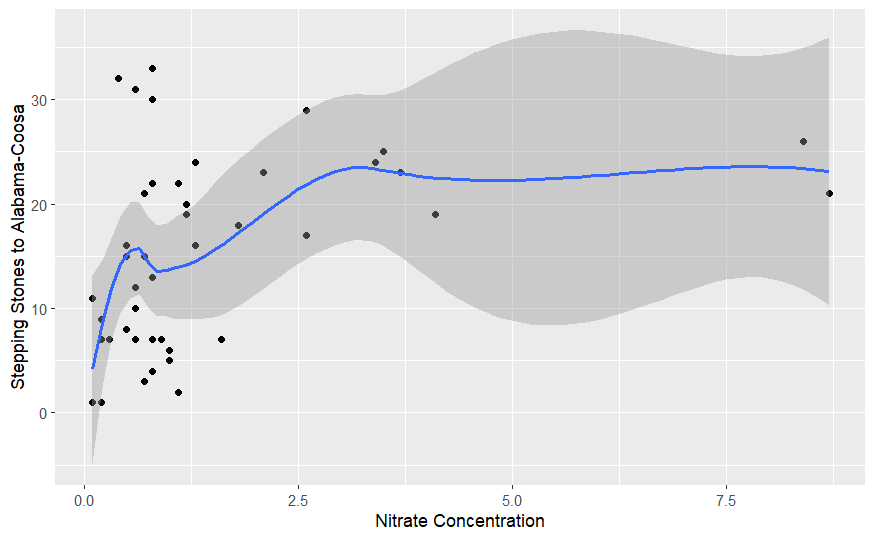
\includegraphics[width=\textwidth]{immagini/ac_nitrate.png}
        \captionsetup{justification=centering}
        \caption{Diagrammma di dispersione tra \texttt{Stepping stones to AC} e \texttt{Nitrate}, con curva LOESS in blu e intervallo di confidenza al 95\% in grigio}
    \end{minipage}
    \hfill
    \begin{minipage}{0.49\textwidth}
        \centering
        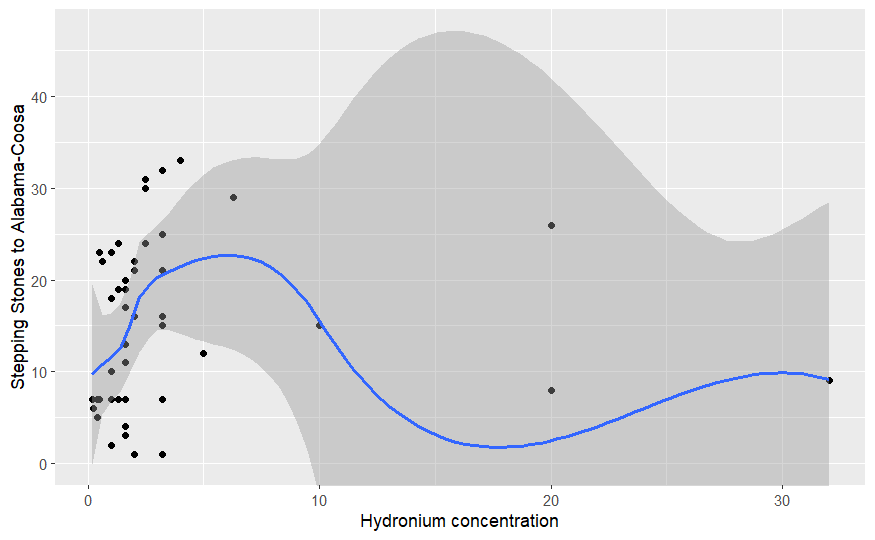
\includegraphics[width=\textwidth]{immagini/ac_hy.png}
        \captionsetup{justification=centering}
        \caption{Diagramma di dispersione tra \texttt{Stepping stones to AC} e \texttt{Hydronium}, con curva LOESS in blu e intervallo di confidenza al 95\% in grigio}
    \end{minipage}
\end{figure}

Dal diagramma di dispersione tra la distanza dei vari fiumi osservati dal sistema fluviale Alabama-Coose e la concentrazione di nitrato nelle acque dei fiumi osservati \textit{(Figura 17)} si osserva una relazione molto curvilinea.
In particolare si nota come i fiumi più vicini al sistema fluviale Alabama-Coose presentano una minore concentrazione di nitrato. La concentrazione di nitrato aumenta all'aumentare della distanza dal sistema fluviale Alabama-Coose, ma solo fino ad un certo punto. Infatti, dopo una certa distanza, la concentrazione di nitrato inizia a diminuire.
La correlazione di Spearman è 0.42, indicando una lieve relazione positiva tra le due variabili. 
Il test per verificare se la correlazione è significativa (S=8173.9, p-value=0.004) porta a rifiutare l'ipotesi che la correlazione non sia significativa.

Dal diagramma di dispersione tra la distanza dei vari fiumi osservati dal sistema fluviale Alabama-Coose e la variabile \texttt{Hydronium} \textit{(Figura 18)} si nota come la maggior parte dei fiumi presenti valori bassi di concentrazione di idronio. Fanno eccezione 5 fiumi che invece presentano valori molto alti di concentrazione di idronio. 
La correlazione di Spearman è 0.33, indicando una lieve relazione positiva tra le due variabili. 
Il test per verificare se la correlazione è significativa (S=9506.5, p-value=0.029) porta a rifiutare l'ipotesi che la correlazione non sia significativa,.

\begin{figure}[H]
    \centering
    \begin{minipage}{0.49\textwidth}
        \centering
        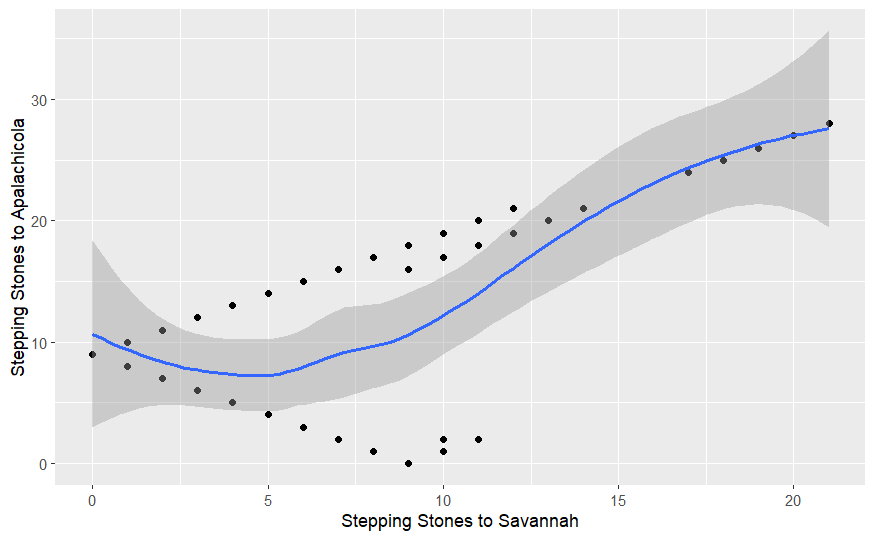
\includegraphics[width=\textwidth]{immagini/ap_sv.png}
        \captionsetup{justification=centering}
        \caption{Diagrammma di dispersione tra \texttt{Stepping stones to AP} e \texttt{Stepping stones to SV}, con curva LOESS in blu e intervallo di confidenza al 95\% in grigio}
    \end{minipage}
    \hfill
    \begin{minipage}{0.49\textwidth}
        \centering
        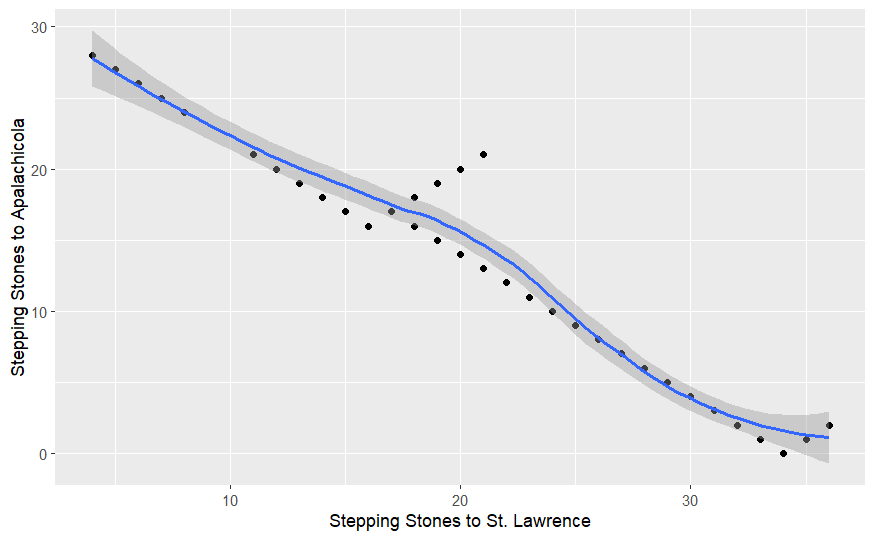
\includegraphics[width=\textwidth]{immagini/ap_sl.png}
        \captionsetup{justification=centering}
        \caption{Diagramma di dispersione tra \texttt{Stepping stones to AP} e \texttt{Stepping stones to SL}, con curva LOESS in blu e intervallo di confidenza al 95\% in grigio}
    \end{minipage}
\end{figure}

Dal diagramma di dispersione tra la distanza dei vari fiumi osservati dal fiume Apalachicola e dal fiume Savannah \textit{(Figura 19)} si nota una relazione tendenzialmente positiva, ma molto curvilinea tra le due variabili. 
Il grafico mostra una situazione simile a quella osservata tra la distanza dei fiumi dal sistema fluviale Alabama-Coose e dal fiume Savannah in \textit{Figura 15}. Anche in questo caso, infatti, si osserva nella prima parte un divergere delle distanze e successivamente un crescere lineare delle stesse. 
Ciò è causato dalla vicinanza del fiume Apalachicola con il sistema fluviale Alabama-Coose, che ne determina un comportamento simile.
La correlazione di Spearman è 0.55, indicando una modesta relazione positiva tra le due variabili.  
Il test per verificare se la correlazione è significativa (S=6436.4, p-value$<$0.001) porta a rifiutare l'ipotesi che la correlazione non sia significativa.

Dal diagramma di dispersione tra la distanza dei vari fiumi osservati dal fiume Apalachicola e dal fiume Saint Lawrence \textit{(Figura 20)} si evince una situazione analoga a quella discussa precedentemente.
Si nota una relazione negativa, abbastanza lineare, tra le due variabili molto simile a quella in \textit{Figura 16}.
La correlazione di Spearman è -0.97, indicando una forte relazione negativa tra le due variabili; dunque all'aumentare della distanza di un fiume dal sistema fluviale Apalachicola diminuisce la distanza dal fiume St. Lawrence. 
Il test per verificare se la correlazione è significativa (S=27892, p-value$<$0.001) porta a rifiutare l'ipotesi che la correlazione non sia significativa.

\begin{figure}[H]
    \centering
    \begin{minipage}{0.49\textwidth}
        \centering
        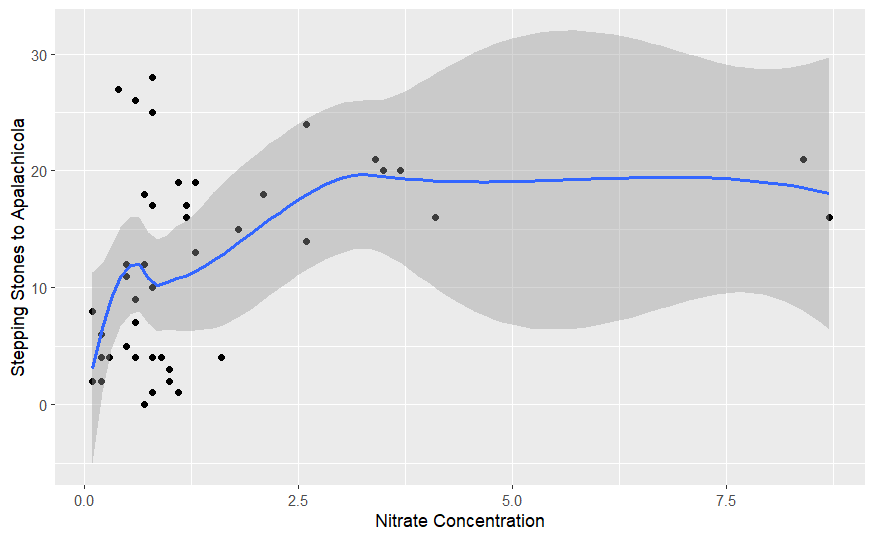
\includegraphics[width=\textwidth]{immagini/ap_nitrate.png}
        \captionsetup{justification=centering}
        \caption{Diagrammma di dispersione tra \texttt{Stepping stones to AP} e \texttt{Nitrate}, con curva LOESS in blu e intervallo di confidenza al 95\% in grigio}
    \end{minipage}
    \hfill
    \begin{minipage}{0.49\textwidth}
        \centering
        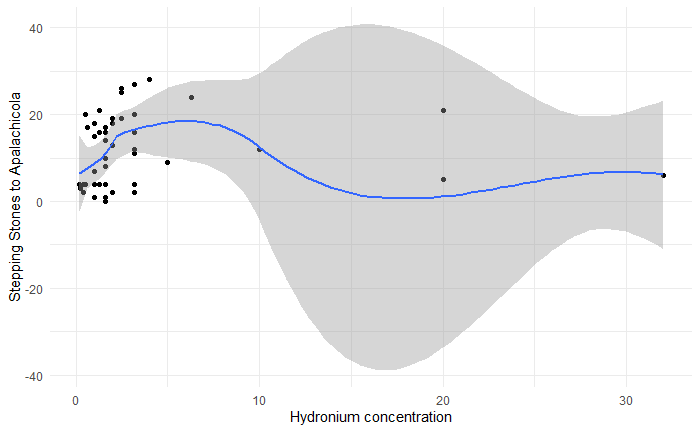
\includegraphics[width=\textwidth]{immagini/ap_hy.png}
        \captionsetup{justification=centering}
        \caption{Diagramma di dispersione tra \texttt{Stepping stones to AP} e \texttt{Hydronium}, con curva LOESS in blu e intervallo di confidenza al 95\% in grigio}
    \end{minipage}
\end{figure}

Dal diagramma di dispersione tra la distanza dei vari fiumi osservati dal fiume Apalachicola e la concentrazione di nitrato nelle acque dei fiumi osservati \textit{(Figura 21)} si nota come i fiumi più vicini al fiume Apalachicola presentano una bassa concentrazione di nitrato, seguita da un aumento di essa mentre ci si allontana dal fiume e infine una diminuzione della concentrazione di nitrato.
La correlazione di Spearman è 0.40, indicando una lieve relazione positiva tra le due variabili. 
Il test per verificare se la correlazione è significativa (S=8454.7, p-value=0.006) porta a rifiutare l'ipotesi che la correlazione non sia significativa.

Dal diagramma di dispersione tra la distanza dei vari fiumi osservati dal fiume Apalachicola e la concentrazione di idronio \textit{(Figura 22)} si nota come la maggior parte dei fiumi sia siutata nella prima parte del grafico, con valori bassi di concentrazione di idronio. Solo 5 fiumi, presentano valori elevati di concentrazione di idronio.
La correlazione di Spearman è 0.33, indicando una lieve relazione positiva tra le due variabili. 
Il test per verificare se la correlazione è significativa (S=9438.8, p-value=0.026) porta a rifiutare l'ipotesi che la correlazione non sia significativa.

\begin{figure}[H]
    \centering
    \begin{minipage}{0.49\textwidth}
        \centering
        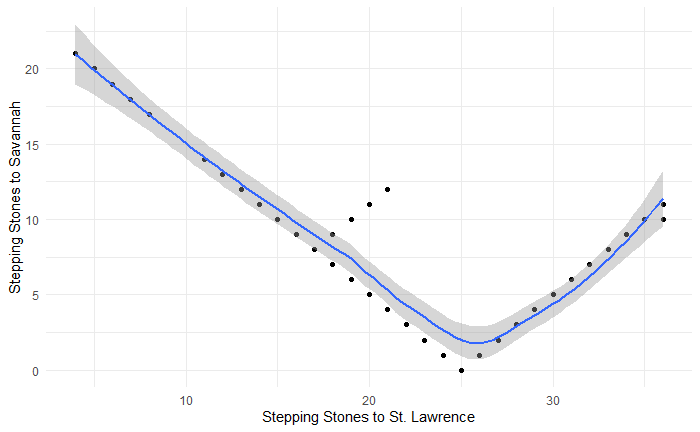
\includegraphics[width=\textwidth]{immagini/sv_sl.png}
        \captionsetup{justification=centering}
        \caption{Diagrammma di dispersione tra \texttt{Stepping stones to SV} e \texttt{Stepping stones to SL}, con curva LOESS in blu e intervallo di confidenza al 95\% in grigio}
    \end{minipage}
    \hfill
    \begin{minipage}{0.49\textwidth}
        \centering
        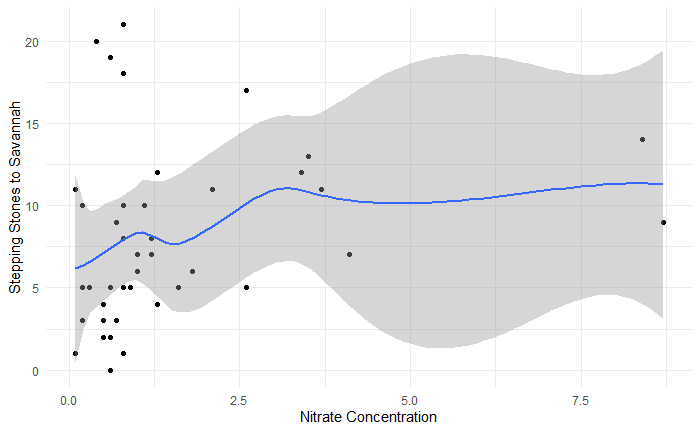
\includegraphics[width=\textwidth]{immagini/sv_nitrate.png}
        \captionsetup{justification=centering}
        \caption{Diagramma di dispersione tra \texttt{Stepping stones to SV} e \texttt{Nitrate}, con curva LOESS in blu e intervallo di confidenza al 95\% in grigio}
    \end{minipage}
\end{figure}

Dal diagramma di dispersione tra la distanza dei vari fiumi osservati dal fiume Savannah e dal fiume St. Lawrence \textit{(Figura 23)} si nota una relazione inizialmente negativa che, una volta raggiunto il fiume Savannah, cambia direzione e cresce positivamente. 
Questo andamento è dovuto alla posizione dei due fiumi. Entrambi i fiumi sfociano nell'Atlantico; il fiume St. Lawrence nasce più a Nord, nella regione dei Grandi Laghi e sfocia in Canada, il fiume Savannah invece è situato più a Sud, in Carolina del Sud. La relazione è inizialmente negativa poiché allontanandosi dal fiume St. Lawrence, e procedendo verso Sud, ci si avvicina al fiume Savannah. Una volta raggiunto il fiume Savannah, le distanze tra i due fiumi aumenteranno in parallelo.
La correlazione di Spearman è -0.51, indicando una relazione negativa tra le due variabili.  
Il test per verificare se la correlazione è significativa (S=21406, p-value=0.0004) porta a rifiutare l'ipotesi che la correlazione non sia significativa.

Dal diagramma di dispersione tra la distanza dei vari fiumi osservati dal fiume Savannah e la concentrazione di nitrato nelle acque dei fiumi osservati \textit{(Figura 24)} si nota un andamento simile a quello della \textit{Figura 17} e della \textit{Figura 21}, anche se la curva LOESS appare meno accentuata. 
Come nella figure precedenti, i fiumi più vicini al fiume Savannah presentano una bassa concentrazione di nitrato, seguita da un suo aumento mentre ci si allontana dal fiume e, infine, una seconda diminuzione della concentrazione di nitrato.
La correlazione di Spearman è 0.36, di poco inferiore a quella tra \texttt{Stepping stones to AC} e \texttt{Nitrate} \texttt{Stepping stones to AP} e \texttt{Nitrate} rispettivamente di 0.42 e 0.40. La relazione è lieve ed è positiva. 
Il test per verificare se la correlazione è significativa (S=9025.2, p-value=0.015) porta a rifiutare l'ipotesi che la correlazione non sia significativa.

\begin{figure}[H]
    \centering
    \begin{minipage}{0.49\textwidth}
        \centering
        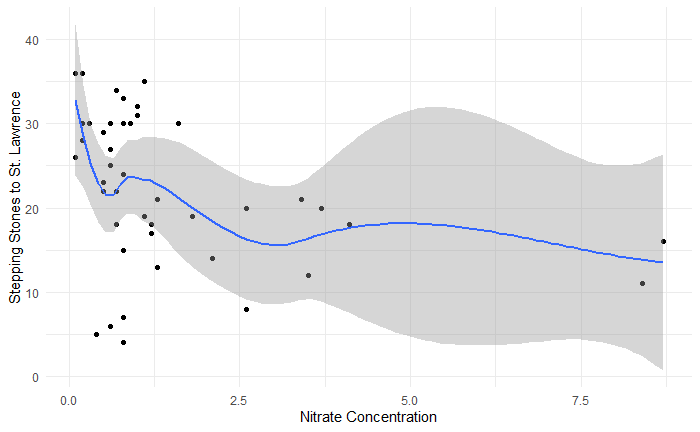
\includegraphics[width=\textwidth]{immagini/sl_nitrate.png}
        \captionsetup{justification=centering}
        \caption{Diagrammma di dispersione tra \texttt{Stepping stones to SL} e \texttt{Nitrate}, con curva LOESS in blu e intervallo di confidenza al 95\% in grigio}
    \end{minipage}
    \hfill
    \begin{minipage}{0.49\textwidth}
        \centering
        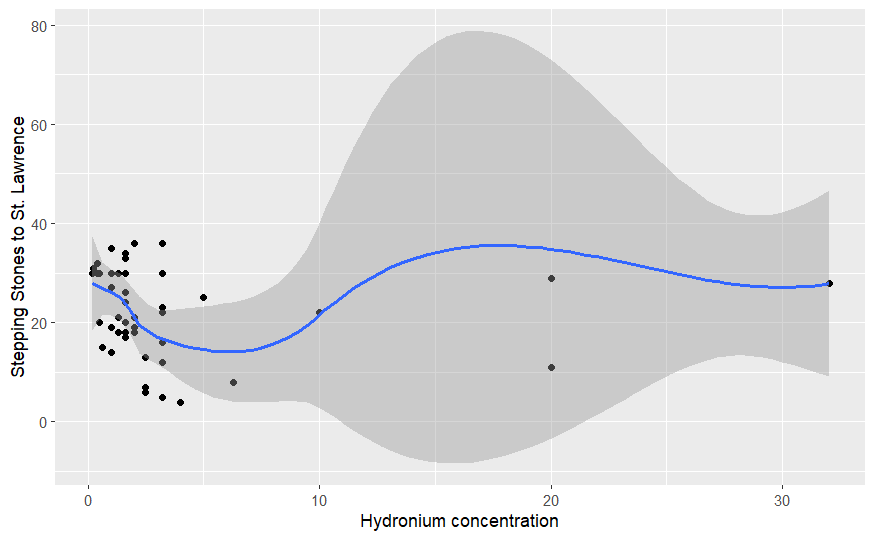
\includegraphics[width=\textwidth]{immagini/sl_hy.png}
        \captionsetup{justification=centering}
        \caption{Diagramma di dispersione tra \texttt{Stepping stones to SL} e \texttt{Hydronium}, con curva LOESS in blu e intervallo di confidenza al 95\% in grigio}
    \end{minipage}
\end{figure}

IL diagramma di dispersione tra la distanza dei vari fiumi osservati dal fiume St. Lawrence e la concentrazione di nitrato nelle acque dei fiumi osservati \textit{(Figura 25)} mostra una situazione capovolta rispetto a quella osservata nelle \textit{Figura 17}, \textit{Figura 21} e \textit{Figura 24}.
Il capovolgimento è dovuto alla posizione più settentrionale del fiume St. Lawrence rispetto agli altri fiumi osservati. I valori che si trovavano distanti dagli altri fiumi, risultano vicini al fiume St. Lawrence e viceversa. 
La correlazione di Spearman è -0.41. La correlazione è negativa, ma, al netto del segno, è in linea con le correlazioni tra gli altri fiumi e la concentrazione di nitrato.  
Il test per verificare se la correlazione è significativa (S=20062, p-value=0.005) porta a rifiutare l'ipotesi che la correlazione non sia significativa.

Dal diagramma di dispersione tra la distanza dei vari fiumi osservati dal fiume St. Lawrence e la concentrazione di idronio \textit{(Figura 26)} si nota come un andamento, analogamente alla \textit{Figura 25}, capovolto rispetto a quello osservata nelle \textit{Figura 18} e \textit{Figura 22}.
La correlazione di Spearman è -0.35, indicando una lieve relazione negativa tra le due variabili. 
Il test per verificare se la correlazione è significativa (S=19135, p-value=0.02) porta a rifiutare l'ipotesi che la correlazione non sia significativa.

\begin{figure}[H]
    \centering
    \begin{minipage}{0.49\textwidth}
        \centering
        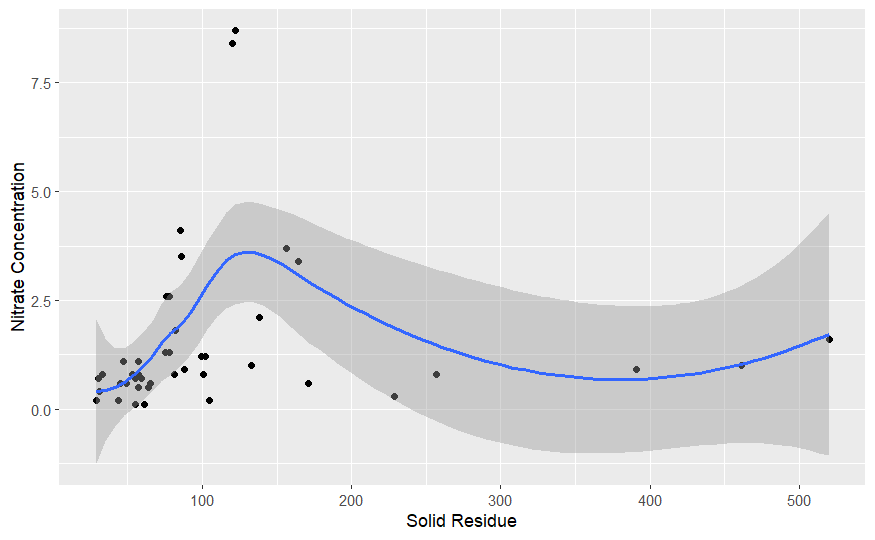
\includegraphics[width=\textwidth]{immagini/sr_nitrate.png}
        \captionsetup{justification=centering}
        \caption{Diagrammma di dispersione tra \texttt{Nitrate} e \texttt{Solid Residue}, con curva LOESS in blu e intervallo di confidenza al 95\% in grigio}
    \end{minipage}
    \hfill
    \begin{minipage}{0.49\textwidth}
        \centering
        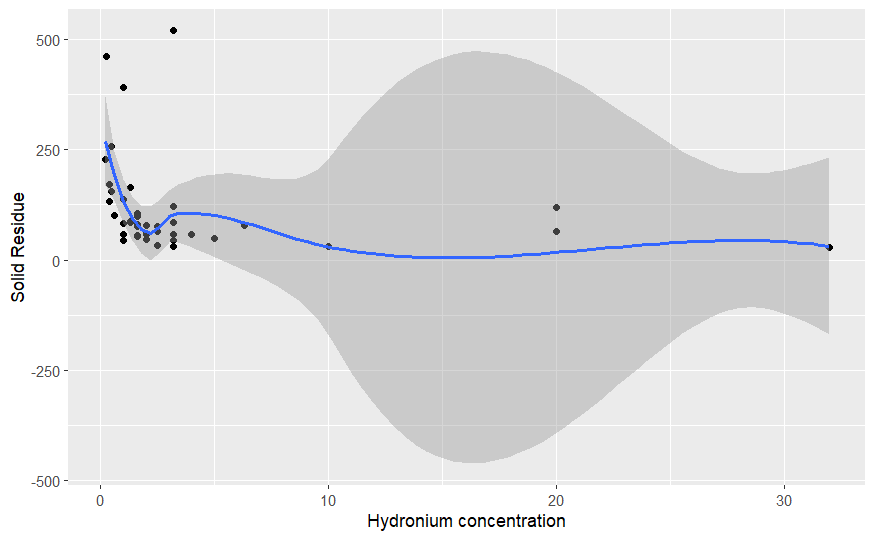
\includegraphics[width=\textwidth]{immagini/sr_hy.png}
        \captionsetup{justification=centering}
        \caption{Diagramma di dispersione tra \texttt{Solid Residue} e \texttt{Hydronium}, con curva LOESS in blu e intervallo di confidenza al 95\% in grigio}
    \end{minipage}
\end{figure}

Dal diagramma di dispersione tra la concentrazione di nitrato e la concentrazione di residuo fisso nelle acque dei fiumi \textit{(Figura 27)} si osserva un iniziale aumento della concentrazione di idronio all'aumentare della concentrazione di residuo fisso. Tuttavia, dopo un certo punto (intorno al valore 150 del residuo fisso), la concentrazione di nitrato inizia a diminuire.
La correlazione di Spearman è 0.50, indicando una modesta relazione positiva tra le due variabili. 
Il test per verificare se la correlazione è significativa (S=7386.3, p-value=0.001) porta a rifiutare l'ipotesi che la correlazione non sia significativa.

Dal diagramma di dispersione tra la concentrazione di residuo fisso e la variabile \texttt{Hydronium} \textit{(Figura 28)} si nota una relazione molto ondulatoria tra le due variabili.
La correlazione è nel complesso (tranne in una piccola parte del grafico tra i valori 2 e 3) negativa.
La correlazione di Spearman è -0.55, confermando la presenza di una modesta relazione negativa tra le due variabili. Dunque, all'aumentare della concentrazione di residuo fisso diminuisce la concentrazione di idronio.
Questo comportamento ha molto senso in quanto nel residuo fisso sono presenti alcuni sali minerali, come bicarbonato (\textit{HCO\textsubscript{3}\textsuperscript{-}}), carbonato (\textit{CO\textsubscript{3}\textsuperscript{2-}}) e cationi metallici (\textit{Ca\textsuperscript{2+}, o Mg\textsuperscript{2+}}) che possono portare ad un effetto tampone, neutralizzando gli ioni idrogeno, e causando una diminuzione della concentrazione di ione idrogeno nell'acqua e, a sua volta, anche del pH.
Il test per verificare se la correlazione è significativa (S=21968, p-value$<$0.001) porta a rifiutare l'ipotesi che la correlazione non sia significativa.

% \newpage
\begin{flushleft}
    \vskip 30pt
    \textbf{\Huge 2. \: Stima del modello}
    \vskip 10pt
    %Prima parte: analisi univariate
    %Titolo
\end{flushleft}

Per stimare il numero di specie di cozze trovate nei vari fiumi, si adattano diversi modelli di regressione. In particolare sono stati valutati un modello lineare multiplo e un modello di Poisson.

\vskip 20pt
\begin{flushleft}
    \textbf{\Large 2.1 \: Modello lineare multiplo}
\end{flushleft}
\vskip 10pt

Come primo modello viene adattato un modello di regressione lineare normale multiplo\textit{[7]}. Il modello è stato ottenuto partendo dal modello saturo: 
\[
Sp =\beta_0+\beta_1 \cdot A+ \beta_2\cdot AC +\beta_3\cdot AP +\beta_4\cdot SV +\beta_5\cdot SL +\beta_6\cdot NO_3 +\beta_7\cdot SR + \beta_8\cdot H^+ +\epsilon_i \quad 
\]
$\text{con } \epsilon_i \sim \mathcal{N}(0,\sigma^2)$\\
dove \textit{Sp} è il numero di specie di cozze, \textit{Area} è l'area di drenaggio, \textit{AC} è la distanza dal fiume Alabama-Coosa, \textit{AP} è la distanza dal fiume Apalachicola, \textit{SV} è la distanza dal fiume Savannah, \textit{SL} è la distanza dal fiume St. Lawrence, \textit{NO\textsubscript{3}} è la concentrazione di nitrato, \textit{SR} è la concentrazione di residuio fisso, \textit{H\textsuperscript{+}} è la concentrazione di ioni di idronio.
È stata utilizzata l'area anziché il suo logaritmo, poiché, usando quest'ultimo, i residui non risultavano normali.
In fase di analisi, seguendo una procedura all'indietro, sono state rimosse in ordine le variabili \texttt{Stepping stones to AC} (p-value = 0.416), \texttt{Stepping stones to SL} (p-value = 0.394), \texttt{nitrate} (p-value = 0.171),   \texttt{Stepping stones to SV} (p-value = 0.134). Il criterio di scelta tra due modelli è stato il criterio di Akaike.

Il modello teorico risultante è:
\[
Sp =\beta_0+\beta_1 \cdot A+\beta_2\cdot AP +\beta_3\cdot SR+\beta_4\cdot H^+ +\epsilon_i \quad \text{con } \epsilon_i \sim \mathcal{N}(0,\sigma^2)
\]
Il vettore dei parametri ignoti di regressione è dato da $(\beta_0,\beta_1,\beta_2,\beta_3,\beta_4)^T$ mentre $\epsilon_i$ rappresenta il termine di errore. 

Il modello stimato è riportato in \textit{Tabella 3}.

\begin{table}[H]
    \centering
    \renewcommand{\arraystretch}{1.4} % Increases the row height
    % \begin{tabularx}{\textwidth}{p{69pt}l p{30pt}c p{45pt}c p{35pt}c p{40pt}c p{30pt}c p{27pt}r}
    \begin{tabular}{lccccc}
        \toprule
        &  Stima &  Std. Error &  2.5\% - 97.5\% (IC) & t-value &  p-value \\
        \midrule  
        \textit{Intercetta} & 15.451   & 1.889  & (11.630, 19.271) & 8.180  & $<$0.001 \\
        \textit{A} & 0.0004   & 0.0001 & (0.0002, 0.0006) & 3.860    & $<$0.001  \\
        \textit{AP} & -0.290   & 0.085  & (-0.462, -0.118)  & -3.415 & 0.002 \\
        \textit{SR} & -0.023   & 0.007  & (-0.037, -0.010) & -3.497 & 0.001  \\
        \textit{H\textsuperscript{+}} & -0.278   & 0.116  & (-0.512, -0.044) & -2.408 & 0.021 \\
        \bottomrule
    \end{tabular}
    \caption{Adattamento del modello lineare multiplo}
\end{table}
Tutti i parametri del modello risultano significativi. 
Il modello stimato risulta:
\[
\hat{Sp}=15.451+0.0004 \cdot A-0.290\cdot AP -0.023\cdot SR-0.278\cdot H^+
\]
Il coefficiente associato  all'area è pari a 0.0004. Questo indica che, per ogni incremento unitario dell'area, si prevede un aumento medio di 0.0004 specie. 
La variabile \texttt{Stepping stones to AP} presenta un coefficiente stimato di -0.290, il che suggerisce che all'aumentare della distanza dal fiume Apalachicola il numero medio di specie diminuisce.
La variabile \texttt{Solid Residue} ha un coefficiente pari a -0.023, indicando che un incremento unitario di \texttt{Solid Residue} comporta una riduzione media di 0.023 specie. Analogamente, la variabile \texttt{Hydronium} ha un coefficiente di -0.278, il che significa che, per ogni incremento unitario di \texttt{Hydronium}, il numero medio di specie diminuisce mediamente di 0.278 \textit{(Tabella 3)}.

\begin{figure}[H]
    \centering
    \begin{minipage}{0.49\textwidth}
        \centering
        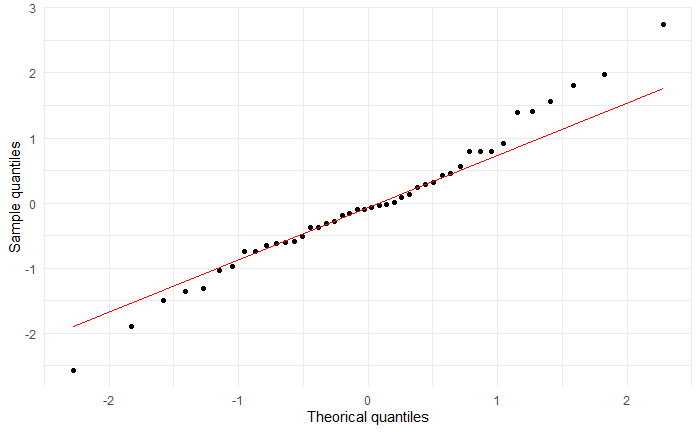
\includegraphics[width=\textwidth]{immagini/qq_lm.png}
        \captionsetup{justification=centering}
        \caption{Diagramma quantile-quantile dei residui del modello}
    \end{minipage}
    \hfill
    \begin{minipage}{0.49\textwidth}
        \centering
        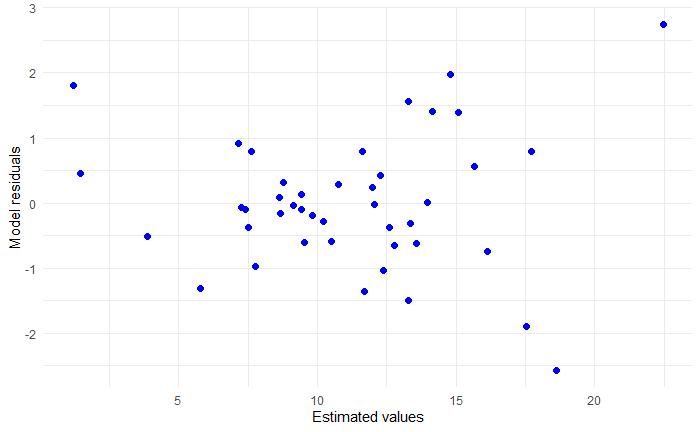
\includegraphics[width=\textwidth]{immagini/res_lm.png}
        \captionsetup{justification=centering}
        \caption{Diagramma di dispersione dei residui rispetto ai valori osservati}
    \end{minipage}
\end{figure}

Sia il diagramma quantile-quantile \textit{(Figura 29)}, sia il test di Shapiro-Wilk (W=0.984, p-value=0.777) confermano l'ipotesi di normalità dei residui del modello stimato. 
Il grafico dei residui studentizzati rispetto ai valori stimati \textit{(Figura 30)} non mostra andamenti sistematici; pertanto, l'ipotesi di omoschedasticità non viene rifiutata. 
L'ipotesi di omogeneità, valutata attraverso la statistica test F, porta a un valore osservato della statistica test pari a 10.63 e un rispettivo p-value prossimo allo zero. Di conseguenza, l'ipotesi è stata rifiutata. 
L'indice di determinazione $R^2$ è pari a 0.522, indicando un moderato adattamento ai dati.

\begin{figure}[H]
    \centering
    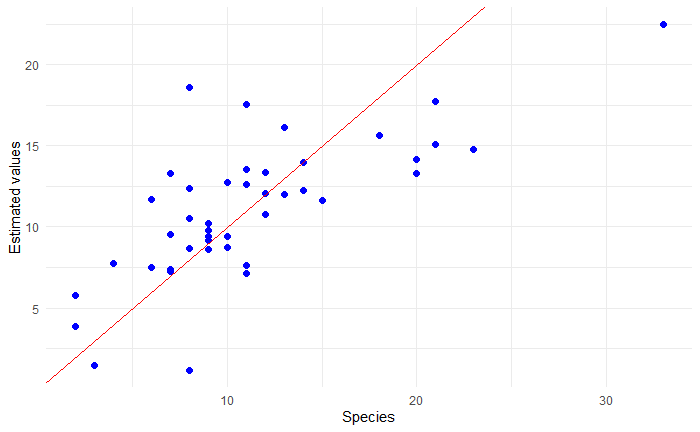
\includegraphics[width=0.5\textwidth]{immagini/res_val_oss_lm.png}
    \captionsetup{justification=centering}
    \caption{Diagramma di dispersione dei \\valori stimati rispetto ai valori osservati}
\end{figure}

Per valutare la bontà di adattamento del modello stimato, si confrontano i valori osservati di \texttt{Species} con quelli predetti dal modello \textit{(Figura 31)}. Il grafico mostra che i punti si distribuiscono principalmente lungo la bisettrice. Questo suggerisce un buon adattamento complessivo del modello ai dati. La correlazione tra i valori osservati e quelli predetti è pari a 0.722, indicando una forte relazione positiva. Questo risultato suggerisce che il modello riesce a spiegare una parte significativa della variabilità del numero di specie.

Nel corso dell'analisi, è stato valutato un modello alternativo in cui la variabile \texttt{Stepping stones to AC} è stata inclusa al posto di \texttt{Stepping stones to AP}. Questa scelta è stata motivata dal fatto che, una volta rimosso il termine \texttt{Stepping stones to AP}, la variabile \texttt{Stepping stones to AC} risultava significativa. Tuttavia, tale modello è stato successivamente scartato in quanto presentava un valore di AIC maggiore (AIC = 261.12) rispetto al modello originale (AIC = 260.918), indicando una minore bontà di adattamento ai dati. Pertanto, si è preferito mantenere il modello iniziale.

\vskip 20pt
\begin{flushleft}
    \textbf{\Large 2.2 \: Modello lineare generalizzato}
\end{flushleft}
\vskip 10pt

Viene adattato un modello lineare generalizzato che assume che la variabile \texttt{Species} segua una distribuzione di Poisson con funzione di legame canonico\textit{[8]}. 
Il modello teorico di partenenza assume che la media sia $\mu_i=e^{\eta_i}$ dove
\[
\eta_i =\alpha_0+\alpha_1 \cdot ln(A)+ \alpha_2\cdot AC +\alpha_3\cdot AP +\alpha_4\cdot SV +\alpha_5\cdot SL +\alpha_6\cdot NO_3 +\alpha_7\cdot SR + \alpha_8\cdot H^+,
\]
Per il modello in esame, è stato adottato il logaritmo dell'area come variabile esplicativa, in quanto questa trasformazione ha portato a un miglioramento del modello. In particolare, rispetto al modello completo con l'area, il valore dell'AIC è diminuito da 245.83 a 241.54, indicando una migliore bontà di adattamento ai dati. Inoltre, la devianza residua è risultata ridotta, passando da 53.801 a 49.509, suggerendo una migliore capacità del modello di spiegare la variabilità del numero di specie.
Anche in questo caso il modello è stato semplificato in fase di analisi seguendo una procedura all'indietro; sono state eliminate le variabili \texttt{Stepping stones to SL} (p-value = 0.829), \texttt{Stepping stones to AC} (p-value = 0.891), \texttt{Stepping stones to SV} (p-value = 0.138), \texttt{Nitrate} (p-value = 0.083).  
Il nuovo modello teorico assume che la media sia $\mu_i=e^{\eta_i}$ dove
\[
\eta_i=\alpha_0+\alpha_1 \cdot ln(A)+\alpha_2\cdot AP +\alpha_3\cdot SR+\alpha_4\cdot H^+ ,
\]
e $(\alpha_0,\alpha_1,\alpha_2,\alpha_3,\alpha_4)^T$ è il vettore dei parametri ignoti di regressione.

Il modello stimato è riportato in \textit{Tabella 4}.
\begin{table}[H]
    \centering
    \renewcommand{\arraystretch}{1.4} % Increases the row height
    % \begin{tabularx}{\textwidth}{p{69pt}l p{30pt}c p{45pt}c p{35pt}c p{40pt}c p{30pt}c p{27pt}r}
    \begin{tabular}{lccccc}
        \toprule
        &  Stima &  Std. Error & 2.5\% - 97.5\% (IC) & t-value &  p-value \\
        \midrule  
            \textit{Intercetta}  & 0.829  & 0.465  & (-0.089, 1.734) & 1.784 & 0.074  \\
            \textit{ln(A)}  & 0.258  & 0.051  & (0.159, 0.358) & 5.098 & $<$0.001 \\
            \textit{AP}  & -0.025 & 0.006  & (-0.036, -0.013) &-4.263 & $<$0.001 \\
            \textit{SR}  & -0.002 & 0.0006 & (-0.003, -0.0009) & -3.376 & $<$0.001 \\
            \textit{H\textsuperscript{+}}  & -0.032 & 0.011  & (-0.055, -0.012) & -2.880 & 0.004 \\
        \bottomrule
    \end{tabular}
    \caption{Adattamento del modello di Poisson}
\end{table}

Tutti i parametri del modello risultano significativi, ad eccezione dell'intercetta.

Il modello stimato risulta:
\[
\log(\hat{\mu}_i)=\hat{\eta_i}=0.829+0.258 \cdot \ln(Area)-0.025\cdot AP -0.002\cdot SR-0.032\cdot H^+
\]

La variabile relativa al logaritmo dell'area ha un coefficiente stimato di 0.258. Questo implica che, per ogni incremento unitario del logaritmo dell'area, il logaritmo del valore atteso della risposta aumenta di 0.258, corrispondendo a un incremento medio del numero di specie di circa $e^{0.258}=1.294$ cioè del $29.4\%$. 
La distanza dal fiume Apalachicola ha un coefficiente pari a -0.0246, indicando che per ogni incremento unitario nella distanza dal fiume il logaritmo del valore atteso della risposta diminuisce di 0.0246, equivalente a una diminuzione media del numero di specie di circa il $2.4\%$.
Per quanto riguarda il residuo fisso, il coefficiente stimato è -0.0021. Questo significa che ogni incremento unitario di residuo fisso determina una diminuzione del logaritmo del valore atteso della risposta di 0.0021, corrispondente a una riduzione media dello $0.2\%$ nel numero di specie.
Infine, la concentrazione di ioni idronio ha un coefficiente stimato di -0.0318. Questo implica che un incremento unitario di idronio riduce il logaritmo del valore atteso della risposta di 0.0318, con una diminuzione media del numero di specie di circa il $3.1\%$ \textit{(Tabella 4)}.

Il test contro il modello nullo porta un valore osservato della statistica test pari a 78.019 e un rispettivo p-value prossimo allo zero, confermando che il modello stimato è significativamente migliore rispetto a quello contenente solo l'intercetta. Inoltre, la devianza residua (49.509) risulta poco maggiore dei gradi di libertà (39), una ulteriore conferma dell'adeguatezza del modello.

\begin{figure}[H]
    \centering
    \begin{minipage}{0.49\textwidth}
        \centering
        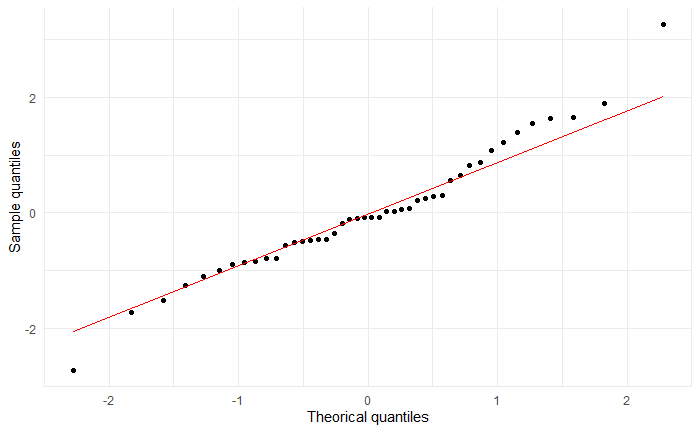
\includegraphics[width=\textwidth]{immagini/qq_glm.png}
        \captionsetup{justification=centering}
        \caption{Diagramma quantile-quantile dei residui del modello}
    \end{minipage}
    \hfill
    \begin{minipage}{0.49\textwidth}
        \centering
        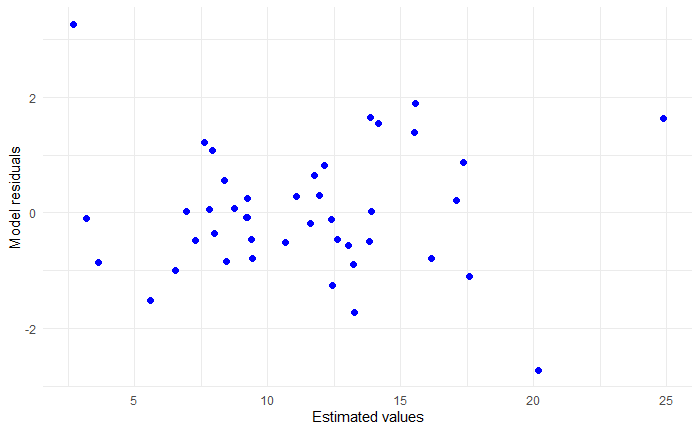
\includegraphics[width=\textwidth]{immagini/res_glm.png}
        \captionsetup{justification=centering}
        \caption{Diagramma di dispersione dei residui rispetto ai valori osservati}
    \end{minipage}
\end{figure}

Sia il diagramma quantile-quantile \textit{(Figura 32)}, sia il test di Shapiro-Wilk (W=0.972, p-value=0.361) confermano l'ipotesi di normalità dei residui del modello stimato. Il grafico dei residui rispetto ai valori stimati \textit{(Figura 33)} non mostra andamenti sistematici; pertanto, l'ipotesi di omoschedasticità non viene rifiutata.

\begin{figure}[H]
    \centering
    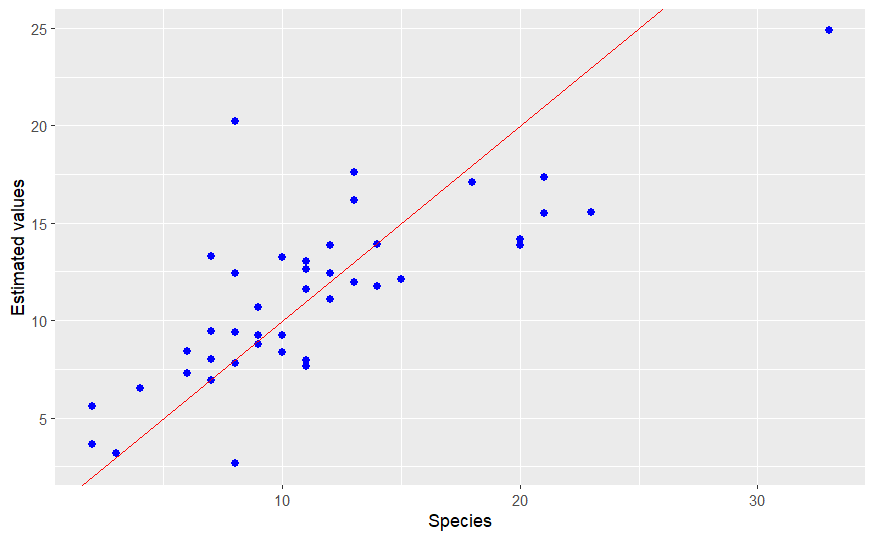
\includegraphics[width=0.5\textwidth]{immagini/res_val_oss_glm.png}
    \captionsetup{justification=centering}
    \caption{Diagramma di dispersione dei \\valori stimati rispetto ai valori osservati}
\end{figure}

Per valutare la bontà di adattamento del modello stimato, sono stati confrontati i valori osservati della variabile \texttt{specie} con quelli predetti dal modello \textit{(Figura 34)}. Il grafico evidenzia che i punti si distribuiscono principalmente lungo la bisettrice. Questo suggerisce un buon adattamento complessivo del modello ai dati. La correlazione tra i valori osservati e quelli predetti è pari a 0.779, indicando una forte relazione positiva. Questo suggerisce che il modello è in grado di spiegare una parte significativa della variabilità nel numero di specie.

Il test per la verifica della sovradispersione restituisce un valore osservato della statistica test pari a 50.568 e un p-value di 0.102; tale ipotesi viene quindi rifiutata.  

Sono state valutate anche altre funzioni di legame, tra cui la radice quadrata ($\eta_i=\sqrt{\mu_i}$) e l'identità ($\eta_i=\mu_i$). Tuttavia, entrambe sono state scartate in quanto presentavano un valore di AIC superiore rispetto a quello del modello con funzione di legame canonica. In particolare, l'AIC del modello con legame canonico è 241.537, mentre quello con legame radice quadrata è 242.206 e quello con legame identità è 243.455.

È stata presa in considerazione la possibilità di includere un termine di interazione tra il numero di \texttt{Stepping stones to AP} e \texttt{area} (p-value = 0.01). Tuttavia, tale termine è stato escluso dal modello, in quanto aveva un coefficiente prossimo allo zero e, data la scarsa numerosità campionaria, non si è voluto appesantire il modello.

È stata considerata l'opportunità di includere un termine di interazione, questa volta tra la distanza dal fiume Apalachicola (\texttt{Stepping stones to AP}) e la concentrazione di idronio (\texttt{Hydronium}) (p-value = 0.001). Tuttavia, si è deciso di non inserirlo, poiché l'analisi dei residui non ha fornito risultati soddisfacenti.


\vskip 30pt
\begin{flushleft}
    \textbf{\Huge 3. \: Conclusioni}
\end{flushleft}
\vskip 10pt

Il numero di specie di cozze è risultato significativamente influenzato dall'area di drenaggio del fiume, dalla distanza dal fiume Apalachicola, dalla quantità di residui fissi in soluzione e dalla concentrazione di ioni idronio.

\begin{figure}[H]
    \centering
    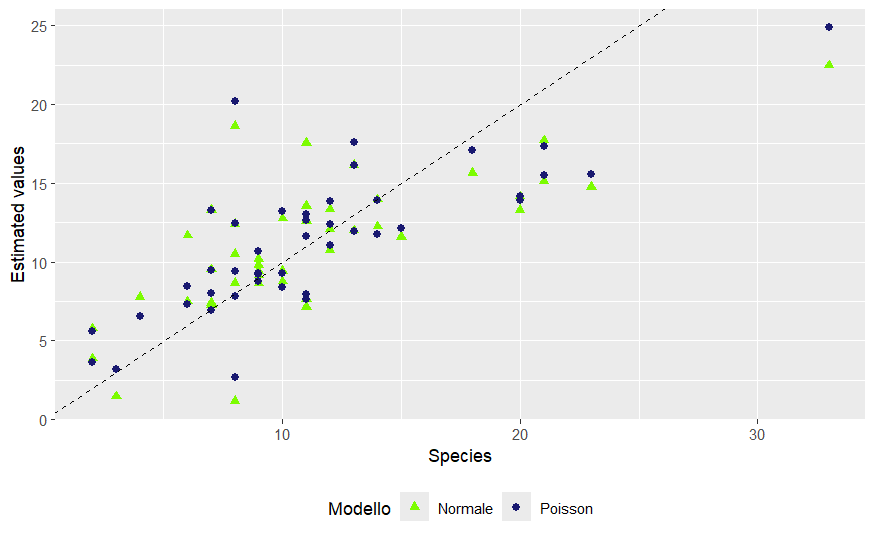
\includegraphics[width=0.7\textwidth]{immagini/lm_glm.png}
    \captionsetup{justification=centering}
    \caption{Diagramma di dispersione tra valori \\osservati e valori predetti con i due modelli}
\end{figure}

Entrambi i modelli stimati mostrano un comportamento complessivamente simile \textit{(Figura 35)}, suggerendo che entrambi riescono a descrivere in modo adeguato le principali relazioni tra le variabili analizzate.

Confrontando gli AIC dei tre modelli, si osserva che il modello di Poisson presenta un valore di AIC inferiore (AIC = 241.537) rispetto al modello lineare normale multiplo (AIC = 260.912). Di conseguenza, in base al criterio di Akaike, si preferisce il modello di Poisson.

Dal punto di vista pratico, i risultati suggeriscono che politiche di conservazione e gestione degli ecosistemi fluviali dovrebbero tenere conto di questi fattori. Ad esempio, la riduzione della concentrazione di ioni idronio (e dunque del ph dell'acqua) e del residuo fisso potrebbe favorire un aumento della biodiversità delle specie di cozze. Inoltre, la vicinanza al fiume Apalachicola sembra svolgere un ruolo chiave nella presenza di un numero maggiore di specie, evidenziando l'importanza di preservare i diversi habitat fluviali.

Data l'importanza ecologica delle cozze di acqua dolce nel corso degli anni sono state oggetto di numerose ricerche.
Esse hanno la capacità di filtrare l'acqua e alcune tossine svolgendo, fondamentalmente, un ruolo di depuratori naturali.
Uno studio condotto nel 1993 sullo stato di conservazione delle cozze di acqua dolce in Stati Uniti e Canada\textit{[9]} ha analizzato 297 specie native, anche a rischio di estinzione, e ha evidenziato alcuni fattori di minaccia per la sopravvivenza delle cozze di acqua dolce come la distruzione dell'habitat causato dalla costruzione di dighe o dal cambiamento dei canali d'acqua e dalla presenza di specie invasive.
Un altro studio, più recente, pubblicato nel 2017 ha analizzato 16 specie di cozze di acqua dolce (2 specie di Margaritiferidae e 14 di Unionidae) in Europa\textit{[10]} e ha evidenziiato ulteriori minacce come la presenza di inquinanti, la scomparsa di pesci ospiti e i pericoli legati al cambiamento climatico. 
Ulteriori sviluppi potrebbero approfondire il ruolo di questi fattori di rischio sulla diffusione delle specie di cozze di acqua dolce. Ci si potrebbe anche concentrare non più solo sul numero di specie, ma anche sulla numerosità della popolazione di ciascuna specie.
O, ancora, dato che il dataset in analisi risale al 1974, uno studio potrebbe essere condotto aggiornando il dataset e valutando l'evoluzione delle specie di cozze di acqua dolce a 40 anni di distanza dallo studio originale.

\begin{spacing}{1.2}
    \newpage
    \begin{flushleft}
        \textbf{\Huge 4. \: Bibliografia}
    \end{flushleft}
    \renewcommand{\refname}{}
    \begin{thebibliography}{9}

    \bibitem{studio_originale}
    Sepkoski J.J, Michael A. (1974). \textit{Distribution of Freshwater Mussels: Coastal Rivers as Biogeographic Islands, Systematic Biology}, Volume 23, Issue 2, Pages 165-188. Rex.

    \bibitem{Mussels_definizione}
    Britannica, T. Editors of Encyclopaedia (2025). \textit{Mussel}. \\https://www.britannica.com/animal/mussel

    \bibitem{nitrate}
    National Center for Biotechnology Information (2025). \textit{PubChem Compound Summary for CID 943, Nitrate}. \\https://pubchem.ncbi.nlm.nih.gov/compound/Nitrate.

    \bibitem{mussels_cibo}
    Indiana Department of Natural Resources (2025). \textit{Freshwater Mussels}. \\https://www.in.gov/dnr/fish-and-wildlife/wildlife-resources/animals/freshwater-mussels/

    \bibitem{shell}
    Pfister C.A., Roy K., Wootton J.T., McCoy S.J., Paine R.T., Suchanek T.H., Sanford E. (2016). \textit{Historical baselines and the future of shell calcification for a foundation species in a changing ocean}. Proc Biol Sci.

    \bibitem{idronio}
    National Center for Biotechnology Information (2025). \textit{PubChem Compound Summary for CID 123332, Oxonium}.\\ https://pubchem.ncbi.nlm.nih.gov/compound/Oxonium.

    \bibitem{modelli_1}
    Grigoletto M., Pauli F., Ventura L. (2017). \textit{Modello Lineare. Teoria e applicazione con R}, Cap 4. Springer.

    \bibitem{modelli_2}
    Salvan A., Sartori N., Pace L. (2020). \textit{Modelli Lineari Generalizzati}, Cap 5. Springer.

    \bibitem{studio_1993}
    Williams J., Jr Melvin, Cummings K., Harris J., Neves R. (1993). \textit{Conservation Status of Freshwater Mussels of The United States and Canada}. Fisheries. 

    \bibitem{studio_2016}
    Lopes-Lima M., Sousa R., Geist J., Aldridge D.C., Araujo R., Bergengren J., Bespalaya Y., Bódis E., Burlakova L., Van Damme D., Douda K., Froufe E., Georgiev D., Gumpinger C., Karatayev A., Kebapçi Ü., Killeen I., Lajtner J., Larsen B.M., Lauceri R., Legakis A., Lois S., Lundberg S., Moorkens E., Motte G., Nagel K.O., Ondina P., Outeiro A., Paunovic M., Prié V., von Proschwitz T., Riccardi N., Rudzīte M., Rudzītis M., Scheder C., Seddon M., Şereflişan H., Simić V., Sokolova S., Stoeckl K., Taskinen J., Teixeira A., Thielen F., Trichkova T., Varandas S., Vicentini H., Zajac K., Zajac T., Zogaris S. (2017). \textit{Conservation status of freshwater mussels in Europe: state of the art and future challenges}. Biol Rev Camb Philos Soc.

    \end{thebibliography}
\end{spacing}
\end{document}